\documentclass[twoside]{book}

% Packages required by doxygen
\usepackage{fixltx2e}
\usepackage{calc}
\usepackage{doxygen}
\usepackage[export]{adjustbox} % also loads graphicx
\usepackage{graphicx}
\usepackage[utf8]{inputenc}
\usepackage{makeidx}
\usepackage{multicol}
\usepackage{multirow}
\PassOptionsToPackage{warn}{textcomp}
\usepackage{textcomp}
\usepackage[nointegrals]{wasysym}
\usepackage[table]{xcolor}

% Font selection
\usepackage[T1]{fontenc}
\usepackage[scaled=.90]{helvet}
\usepackage{courier}
\usepackage{amssymb}
\usepackage{sectsty}
\renewcommand{\familydefault}{\sfdefault}
\allsectionsfont{%
  \fontseries{bc}\selectfont%
  \color{darkgray}%
}
\renewcommand{\DoxyLabelFont}{%
  \fontseries{bc}\selectfont%
  \color{darkgray}%
}
\newcommand{\+}{\discretionary{\mbox{\scriptsize$\hookleftarrow$}}{}{}}

% Page & text layout
\usepackage{geometry}
\geometry{%
  a4paper,%
  top=2.5cm,%
  bottom=2.5cm,%
  left=2.5cm,%
  right=2.5cm%
}
\tolerance=750
\hfuzz=15pt
\hbadness=750
\setlength{\emergencystretch}{15pt}
\setlength{\parindent}{0cm}
\setlength{\parskip}{0.2cm}
\makeatletter
\renewcommand{\paragraph}{%
  \@startsection{paragraph}{4}{0ex}{-1.0ex}{1.0ex}{%
    \normalfont\normalsize\bfseries\SS@parafont%
  }%
}
\renewcommand{\subparagraph}{%
  \@startsection{subparagraph}{5}{0ex}{-1.0ex}{1.0ex}{%
    \normalfont\normalsize\bfseries\SS@subparafont%
  }%
}
\makeatother

% Headers & footers
\usepackage{fancyhdr}
\pagestyle{fancyplain}
\fancyhead[LE]{\fancyplain{}{\bfseries\thepage}}
\fancyhead[CE]{\fancyplain{}{}}
\fancyhead[RE]{\fancyplain{}{\bfseries\leftmark}}
\fancyhead[LO]{\fancyplain{}{\bfseries\rightmark}}
\fancyhead[CO]{\fancyplain{}{}}
\fancyhead[RO]{\fancyplain{}{\bfseries\thepage}}
\fancyfoot[LE]{\fancyplain{}{}}
\fancyfoot[CE]{\fancyplain{}{}}
\fancyfoot[RE]{\fancyplain{}{\bfseries\scriptsize Generated on Tue May 5 2015 15\+:51\+:30 for My Project by Doxygen }}
\fancyfoot[LO]{\fancyplain{}{\bfseries\scriptsize Generated on Tue May 5 2015 15\+:51\+:30 for My Project by Doxygen }}
\fancyfoot[CO]{\fancyplain{}{}}
\fancyfoot[RO]{\fancyplain{}{}}
\renewcommand{\footrulewidth}{0.4pt}
\renewcommand{\chaptermark}[1]{%
  \markboth{#1}{}%
}
\renewcommand{\sectionmark}[1]{%
  \markright{\thesection\ #1}%
}

% Indices & bibliography
\usepackage{natbib}
\usepackage[titles]{tocloft}
\setcounter{tocdepth}{3}
\setcounter{secnumdepth}{5}
\makeindex

% Hyperlinks (required, but should be loaded last)
\usepackage{ifpdf}
\ifpdf
  \usepackage[pdftex,pagebackref=true]{hyperref}
\else
  \usepackage[ps2pdf,pagebackref=true]{hyperref}
\fi
\hypersetup{%
  colorlinks=true,%
  linkcolor=blue,%
  citecolor=blue,%
  unicode%
}

% Custom commands
\newcommand{\clearemptydoublepage}{%
  \newpage{\pagestyle{empty}\cleardoublepage}%
}


%===== C O N T E N T S =====

\begin{document}

% Titlepage & ToC
\hypersetup{pageanchor=false,
             bookmarks=true,
             bookmarksnumbered=true,
             pdfencoding=unicode
            }
\pagenumbering{roman}
\begin{titlepage}
\vspace*{7cm}
\begin{center}%
{\Large My Project }\\
\vspace*{1cm}
{\large Generated by Doxygen 1.8.9.1}\\
\vspace*{0.5cm}
{\small Tue May 5 2015 15:51:30}\\
\end{center}
\end{titlepage}
\clearemptydoublepage
\tableofcontents
\clearemptydoublepage
\pagenumbering{arabic}
\hypersetup{pageanchor=true}

%--- Begin generated contents ---
\chapter{Hierarchical Index}
\section{Class Hierarchy}
This inheritance list is sorted roughly, but not completely, alphabetically\+:\begin{DoxyCompactList}
\item \contentsline{section}{comp\+Time}{\pageref{classcompTime}}{}
\item \contentsline{section}{Diff\+Eq\+\_\+\+Sim}{\pageref{classDiffEq__Sim}}{}
\begin{DoxyCompactList}
\item \contentsline{section}{Deterministic\+\_\+\+Network\+\_\+\+S\+I\+R\+\_\+\+Sim}{\pageref{classDeterministic__Network__SIR__Sim}}{}
\item \contentsline{section}{S\+I\+R}{\pageref{classSIR}}{}
\end{DoxyCompactList}
\item \contentsline{section}{Edge}{\pageref{classEdge}}{}
\item \contentsline{section}{Event}{\pageref{classEvent}}{}
\item \contentsline{section}{Gillespie\+\_\+\+Mass\+Action\+\_\+\+Sim}{\pageref{classGillespie__MassAction__Sim}}{}
\item \contentsline{section}{Gillespie\+\_\+\+Network\+\_\+\+S\+E\+I\+R\+S\+\_\+\+Sim}{\pageref{classGillespie__Network__SEIRS__Sim}}{}
\item \contentsline{section}{Intervention}{\pageref{classIntervention}}{}
\item \contentsline{section}{M\+T\+Rand}{\pageref{classMTRand}}{}
\item \contentsline{section}{Network}{\pageref{classNetwork}}{}
\item \contentsline{section}{Node}{\pageref{classNode}}{}
\item \contentsline{section}{R\+Plot}{\pageref{classRPlot}}{}
\item \contentsline{section}{Simulator}{\pageref{classSimulator}}{}
\begin{DoxyCompactList}
\item \contentsline{section}{Chain\+Binomial\+\_\+\+Sim}{\pageref{classChainBinomial__Sim}}{}
\item \contentsline{section}{Opinion\+\_\+formation}{\pageref{classOpinion__formation}}{}
\item \contentsline{section}{Percolation\+\_\+\+Sim}{\pageref{classPercolation__Sim}}{}
\end{DoxyCompactList}
\item \contentsline{section}{Trigger}{\pageref{classTrigger}}{}
\item \contentsline{section}{Yseries}{\pageref{classYseries}}{}
\end{DoxyCompactList}

\chapter{Class Index}
\section{Class List}
Here are the classes, structs, unions and interfaces with brief descriptions\+:\begin{DoxyCompactList}
\item\contentsline{section}{\hyperlink{classChainBinomial__Sim}{Chain\+Binomial\+\_\+\+Sim} }{\pageref{classChainBinomial__Sim}}{}
\item\contentsline{section}{\hyperlink{classcompTime}{comp\+Time} }{\pageref{classcompTime}}{}
\item\contentsline{section}{\hyperlink{classDeterministic__Network__SIR__Sim}{Deterministic\+\_\+\+Network\+\_\+\+S\+I\+R\+\_\+\+Sim} }{\pageref{classDeterministic__Network__SIR__Sim}}{}
\item\contentsline{section}{\hyperlink{classDiffEq__Sim}{Diff\+Eq\+\_\+\+Sim} }{\pageref{classDiffEq__Sim}}{}
\item\contentsline{section}{\hyperlink{classEdge}{Edge} }{\pageref{classEdge}}{}
\item\contentsline{section}{\hyperlink{classEvent}{Event} }{\pageref{classEvent}}{}
\item\contentsline{section}{\hyperlink{classGillespie__MassAction__Sim}{Gillespie\+\_\+\+Mass\+Action\+\_\+\+Sim} }{\pageref{classGillespie__MassAction__Sim}}{}
\item\contentsline{section}{\hyperlink{classGillespie__Network__SEIRS__Sim}{Gillespie\+\_\+\+Network\+\_\+\+S\+E\+I\+R\+S\+\_\+\+Sim} }{\pageref{classGillespie__Network__SEIRS__Sim}}{}
\item\contentsline{section}{\hyperlink{classIntervention}{Intervention} }{\pageref{classIntervention}}{}
\item\contentsline{section}{\hyperlink{classMTRand}{M\+T\+Rand} }{\pageref{classMTRand}}{}
\item\contentsline{section}{\hyperlink{classNetwork}{Network} }{\pageref{classNetwork}}{}
\item\contentsline{section}{\hyperlink{classNode}{Node} }{\pageref{classNode}}{}
\item\contentsline{section}{\hyperlink{classOpinion__formation}{Opinion\+\_\+formation} }{\pageref{classOpinion__formation}}{}
\item\contentsline{section}{\hyperlink{classPercolation__Sim}{Percolation\+\_\+\+Sim} }{\pageref{classPercolation__Sim}}{}
\item\contentsline{section}{\hyperlink{classRPlot}{R\+Plot} }{\pageref{classRPlot}}{}
\item\contentsline{section}{\hyperlink{classSimulator}{Simulator} }{\pageref{classSimulator}}{}
\item\contentsline{section}{\hyperlink{classSIR}{S\+I\+R} }{\pageref{classSIR}}{}
\item\contentsline{section}{\hyperlink{classTrigger}{Trigger} }{\pageref{classTrigger}}{}
\item\contentsline{section}{\hyperlink{classYseries}{Yseries} }{\pageref{classYseries}}{}
\end{DoxyCompactList}

\chapter{Class Documentation}
\hypertarget{classChainBinomial__Sim}{}\section{Chain\+Binomial\+\_\+\+Sim Class Reference}
\label{classChainBinomial__Sim}\index{Chain\+Binomial\+\_\+\+Sim@{Chain\+Binomial\+\_\+\+Sim}}
Inheritance diagram for Chain\+Binomial\+\_\+\+Sim\+:\begin{figure}[H]
\begin{center}
\leavevmode
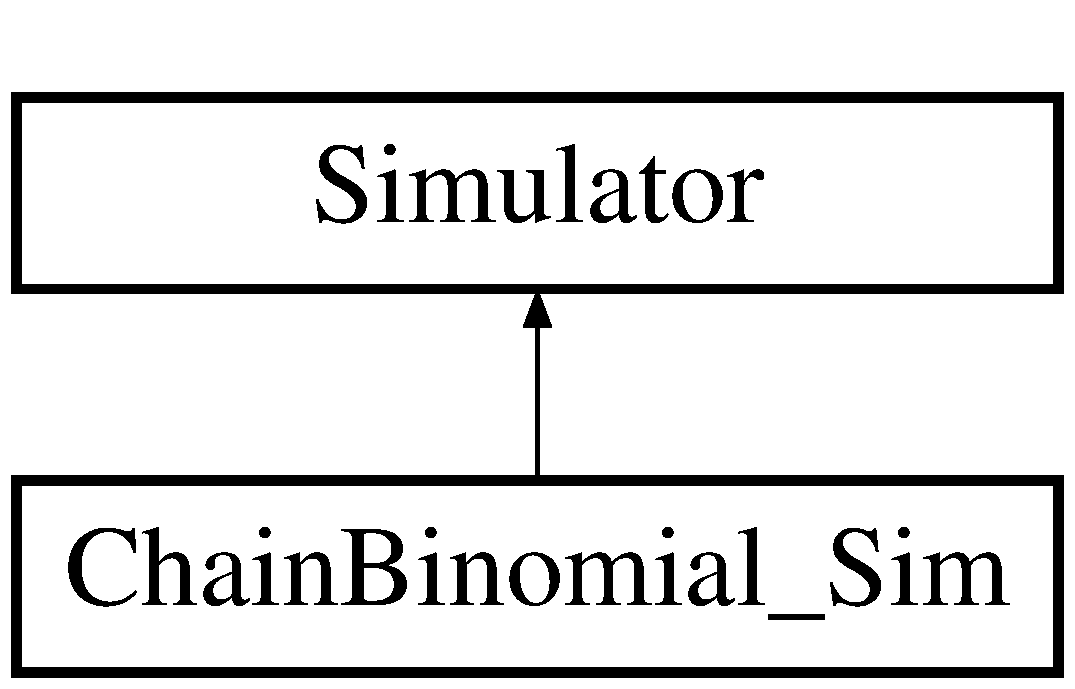
\includegraphics[height=2.000000cm]{classChainBinomial__Sim}
\end{center}
\end{figure}
\subsection*{Public Member Functions}
\begin{DoxyCompactItemize}
\item 
\hypertarget{classChainBinomial__Sim_a3d8360a4accc75a1fd05358cfea134c7}{}{\bfseries Chain\+Binomial\+\_\+\+Sim} (\hyperlink{classNetwork}{Network} $\ast$net, int infectious\+\_\+period, double T)\label{classChainBinomial__Sim_a3d8360a4accc75a1fd05358cfea134c7}

\item 
\hypertarget{classChainBinomial__Sim_a7194af935f019e49e73858f726fb7db3}{}void {\bfseries set\+\_\+network} (\hyperlink{classNetwork}{Network} $\ast$net)\label{classChainBinomial__Sim_a7194af935f019e49e73858f726fb7db3}

\item 
\hypertarget{classChainBinomial__Sim_acb28925f5ef15976df7bd74bb5f475f5}{}void {\bfseries set\+\_\+infectious\+\_\+period} (int d)\label{classChainBinomial__Sim_acb28925f5ef15976df7bd74bb5f475f5}

\item 
\hypertarget{classChainBinomial__Sim_a42bcc404ba9b7fa3dfe09bc261c18555}{}void {\bfseries set\+\_\+transmissibility} (double t)\label{classChainBinomial__Sim_a42bcc404ba9b7fa3dfe09bc261c18555}

\item 
\hypertarget{classChainBinomial__Sim_a20bc89bd36f687b0fbf26eb0d791c942}{}vector$<$ double $>$ {\bfseries define\+\_\+time\+\_\+dist} ()\label{classChainBinomial__Sim_a20bc89bd36f687b0fbf26eb0d791c942}

\item 
\hypertarget{classChainBinomial__Sim_a170153814fa16f65545aa9d84efc5d8a}{}int {\bfseries get\+\_\+infectious\+\_\+period} ()\label{classChainBinomial__Sim_a170153814fa16f65545aa9d84efc5d8a}

\item 
\hypertarget{classChainBinomial__Sim_af3a446813e5877097ae19eef01f42035}{}double {\bfseries get\+\_\+transmissibility} ()\label{classChainBinomial__Sim_af3a446813e5877097ae19eef01f42035}

\item 
\hypertarget{classChainBinomial__Sim_a014207862000aa1ce033f151fa8bee66}{}vector$<$ \hyperlink{classNode}{Node} $\ast$ $>$ {\bfseries rand\+\_\+infect} (int n)\label{classChainBinomial__Sim_a014207862000aa1ce033f151fa8bee66}

\item 
\hypertarget{classChainBinomial__Sim_a3c4c019ab2f85962c28fe3dd85ee08ef}{}void {\bfseries infect\+\_\+node} (\hyperlink{classNode}{Node} $\ast$node)\label{classChainBinomial__Sim_a3c4c019ab2f85962c28fe3dd85ee08ef}

\item 
\hypertarget{classChainBinomial__Sim_affb5dba83fcb57724462b56fb0695ce0}{}void {\bfseries step\+\_\+simulation} ()\label{classChainBinomial__Sim_affb5dba83fcb57724462b56fb0695ce0}

\item 
\hypertarget{classChainBinomial__Sim_a1dc4e4eedec788c0d783fbb8b6a70308}{}void {\bfseries run\+\_\+simulation} ()\label{classChainBinomial__Sim_a1dc4e4eedec788c0d783fbb8b6a70308}

\item 
\hypertarget{classChainBinomial__Sim_a8d62910cfad67fe05f3a5de667ed6f9b}{}void {\bfseries add\+\_\+event} (\hyperlink{classNode}{Node} $\ast$sink\+\_\+node, int time, \hyperlink{classNode}{Node} $\ast$source\+\_\+node)\label{classChainBinomial__Sim_a8d62910cfad67fe05f3a5de667ed6f9b}

\item 
\hypertarget{classChainBinomial__Sim_aea23cd4cc94a78132e16c0eefcd70c71}{}int {\bfseries count\+\_\+infected} ()\label{classChainBinomial__Sim_aea23cd4cc94a78132e16c0eefcd70c71}

\item 
\hypertarget{classChainBinomial__Sim_afd59eb923a3c287787d914fc7d77c60f}{}int {\bfseries epidemic\+\_\+size} ()\label{classChainBinomial__Sim_afd59eb923a3c287787d914fc7d77c60f}

\item 
\hypertarget{classChainBinomial__Sim_a837114b07c1655f241db8e31190289f6}{}vector$<$ int $>$ {\bfseries get\+\_\+epi\+\_\+curve} ()\label{classChainBinomial__Sim_a837114b07c1655f241db8e31190289f6}

\item 
\hypertarget{classChainBinomial__Sim_ac9d248964bc52237ae9698a0e1ca40af}{}vector$<$ int $>$ {\bfseries get\+\_\+prevalence\+\_\+curve} ()\label{classChainBinomial__Sim_ac9d248964bc52237ae9698a0e1ca40af}

\item 
\hypertarget{classChainBinomial__Sim_a5e475fcdaca86cb4467f4c17e3240217}{}vector$<$ pair$<$ int, \hyperlink{classNode}{Node} $\ast$ $>$ $>$ {\bfseries get\+\_\+detailed\+\_\+epi\+\_\+curve} ()\label{classChainBinomial__Sim_a5e475fcdaca86cb4467f4c17e3240217}

\item 
\hypertarget{classChainBinomial__Sim_ad3be9818d5389bd0b507248454968a2a}{}void {\bfseries reset} ()\label{classChainBinomial__Sim_ad3be9818d5389bd0b507248454968a2a}

\item 
\hypertarget{classChainBinomial__Sim_abbdf731e6bdb9af8f17eac392ba81a6f}{}void {\bfseries summary} ()\label{classChainBinomial__Sim_abbdf731e6bdb9af8f17eac392ba81a6f}

\end{DoxyCompactItemize}
\subsection*{Public Attributes}
\begin{DoxyCompactItemize}
\item 
\hypertarget{classChainBinomial__Sim_a17cd2e68f958b9b818dc061221dca6cb}{}double {\bfseries T}\label{classChainBinomial__Sim_a17cd2e68f958b9b818dc061221dca6cb}

\item 
\hypertarget{classChainBinomial__Sim_a94ddda2a0fa2a307e094e555d739b3e0}{}int {\bfseries infectious\+\_\+period}\label{classChainBinomial__Sim_a94ddda2a0fa2a307e094e555d739b3e0}

\end{DoxyCompactItemize}
\subsection*{Protected Attributes}
\begin{DoxyCompactItemize}
\item 
\hypertarget{classChainBinomial__Sim_a28b17a028f8540dd8c9eea9b4afd8dc3}{}list$<$ \hyperlink{classNode}{Node} $\ast$ $>$ {\bfseries infected}\label{classChainBinomial__Sim_a28b17a028f8540dd8c9eea9b4afd8dc3}

\item 
\hypertarget{classChainBinomial__Sim_a6f871e9e85e4dbf5dd8704d8e114adc9}{}vector$<$ \hyperlink{classNode}{Node} $\ast$ $>$ {\bfseries recovered}\label{classChainBinomial__Sim_a6f871e9e85e4dbf5dd8704d8e114adc9}

\item 
\hypertarget{classChainBinomial__Sim_a3bf87d7371bb0d354ef9d8fe19c2ba50}{}vector$<$ double $>$ {\bfseries time\+\_\+dist}\label{classChainBinomial__Sim_a3bf87d7371bb0d354ef9d8fe19c2ba50}

\item 
\hypertarget{classChainBinomial__Sim_a897837a54e9fccf9b6b8e4c0d4d66ca9}{}bool {\bfseries update\+\_\+time\+\_\+dist}\label{classChainBinomial__Sim_a897837a54e9fccf9b6b8e4c0d4d66ca9}

\item 
\hypertarget{classChainBinomial__Sim_ae0b621ed8981260be2c0b77587f847cc}{}priority\+\_\+queue$<$ \hyperlink{classEvent}{Event}, vector$<$ \hyperlink{classEvent}{Event} $>$, \hyperlink{classcompTime}{comp\+Time} $>$ {\bfseries transmission\+Q}\label{classChainBinomial__Sim_ae0b621ed8981260be2c0b77587f847cc}

\item 
\hypertarget{classChainBinomial__Sim_a78b56d1a4485d37390fc017715763381}{}vector$<$ int $>$ {\bfseries epi\+\_\+curve}\label{classChainBinomial__Sim_a78b56d1a4485d37390fc017715763381}

\item 
\hypertarget{classChainBinomial__Sim_a321ab6e9f586ec9013f2cc8ecd1cf03b}{}vector$<$ pair$<$ int, \hyperlink{classNode}{Node} $\ast$ $>$ $>$ {\bfseries detailed\+\_\+epi\+\_\+curve}\label{classChainBinomial__Sim_a321ab6e9f586ec9013f2cc8ecd1cf03b}

\end{DoxyCompactItemize}


The documentation for this class was generated from the following file\+:\begin{DoxyCompactItemize}
\item 
Chain\+Binomial\+\_\+\+Sim.\+h\end{DoxyCompactItemize}

\hypertarget{classcompTime}{}\section{comp\+Time Class Reference}
\label{classcompTime}\index{comp\+Time@{comp\+Time}}
\subsection*{Public Member Functions}
\begin{DoxyCompactItemize}
\item 
\hypertarget{classcompTime_a55a31c09678c7121976d07a5b46c9ef0}{}bool {\bfseries operator()} (const \hyperlink{classEvent}{Event} $\ast$lhs, const \hyperlink{classEvent}{Event} $\ast$rhs) const \label{classcompTime_a55a31c09678c7121976d07a5b46c9ef0}

\item 
\hypertarget{classcompTime_ada86cc3bfdd095db80a56254f5ecacf2}{}bool {\bfseries operator()} (const \hyperlink{classEvent}{Event} \&lhs, const \hyperlink{classEvent}{Event} \&rhs) const \label{classcompTime_ada86cc3bfdd095db80a56254f5ecacf2}

\item 
\hypertarget{classcompTime_a55a31c09678c7121976d07a5b46c9ef0}{}bool {\bfseries operator()} (const \hyperlink{classEvent}{Event} $\ast$lhs, const \hyperlink{classEvent}{Event} $\ast$rhs) const \label{classcompTime_a55a31c09678c7121976d07a5b46c9ef0}

\item 
\hypertarget{classcompTime_ada86cc3bfdd095db80a56254f5ecacf2}{}bool {\bfseries operator()} (const \hyperlink{classEvent}{Event} \&lhs, const \hyperlink{classEvent}{Event} \&rhs) const \label{classcompTime_ada86cc3bfdd095db80a56254f5ecacf2}

\item 
\hypertarget{classcompTime_a55a31c09678c7121976d07a5b46c9ef0}{}bool {\bfseries operator()} (const \hyperlink{classEvent}{Event} $\ast$lhs, const \hyperlink{classEvent}{Event} $\ast$rhs) const \label{classcompTime_a55a31c09678c7121976d07a5b46c9ef0}

\item 
\hypertarget{classcompTime_ada86cc3bfdd095db80a56254f5ecacf2}{}bool {\bfseries operator()} (const \hyperlink{classEvent}{Event} \&lhs, const \hyperlink{classEvent}{Event} \&rhs) const \label{classcompTime_ada86cc3bfdd095db80a56254f5ecacf2}

\end{DoxyCompactItemize}


The documentation for this class was generated from the following files\+:\begin{DoxyCompactItemize}
\item 
Chain\+Binomial\+\_\+\+Sim.\+h\item 
Gillespie\+\_\+\+Mass\+Action\+\_\+\+Sim.\+h\item 
Gillespie\+\_\+\+Network\+\_\+\+S\+E\+I\+R\+S\+\_\+\+Sim.\+h\end{DoxyCompactItemize}

\hypertarget{classDeterministic__Network__SIR__Sim}{}\section{Deterministic\+\_\+\+Network\+\_\+\+S\+I\+R\+\_\+\+Sim Class Reference}
\label{classDeterministic__Network__SIR__Sim}\index{Deterministic\+\_\+\+Network\+\_\+\+S\+I\+R\+\_\+\+Sim@{Deterministic\+\_\+\+Network\+\_\+\+S\+I\+R\+\_\+\+Sim}}
Inheritance diagram for Deterministic\+\_\+\+Network\+\_\+\+S\+I\+R\+\_\+\+Sim\+:\begin{figure}[H]
\begin{center}
\leavevmode
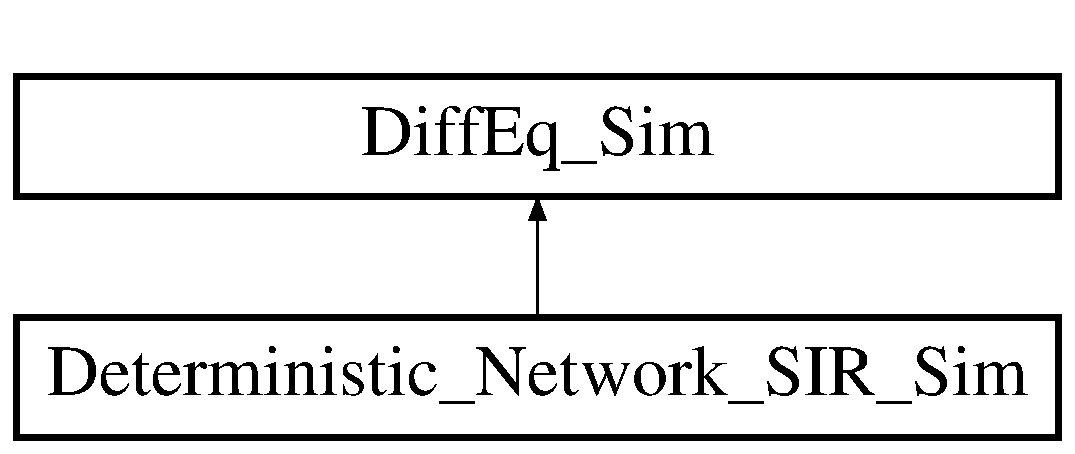
\includegraphics[height=2.000000cm]{classDeterministic__Network__SIR__Sim}
\end{center}
\end{figure}
\subsection*{Public Member Functions}
\begin{DoxyCompactItemize}
\item 
\hypertarget{classDeterministic__Network__SIR__Sim_ab65875e06295f845030460b4c402f9d7}{}{\bfseries Deterministic\+\_\+\+Network\+\_\+\+S\+I\+R\+\_\+\+Sim} (double r\+\_\+param, double mu\+\_\+param, vector$<$ double $>$ deg\+\_\+dist\+\_\+param)\label{classDeterministic__Network__SIR__Sim_ab65875e06295f845030460b4c402f9d7}

\item 
\hypertarget{classDeterministic__Network__SIR__Sim_a87a198e25b592969ffda784290816ab8}{}void {\bfseries initialize} (double theta, double p\+S, double p\+I, double I)\label{classDeterministic__Network__SIR__Sim_a87a198e25b592969ffda784290816ab8}

\item 
\hypertarget{classDeterministic__Network__SIR__Sim_a35e200c2f3647ec2127425a4fa97a6ec}{}double {\bfseries current\+\_\+susceptible} ()\label{classDeterministic__Network__SIR__Sim_a35e200c2f3647ec2127425a4fa97a6ec}

\item 
\hypertarget{classDeterministic__Network__SIR__Sim_af69a8b7222a167f184dfaf8c808562fe}{}double {\bfseries current\+\_\+infectious} ()\label{classDeterministic__Network__SIR__Sim_af69a8b7222a167f184dfaf8c808562fe}

\item 
\hypertarget{classDeterministic__Network__SIR__Sim_abf76f121a50f0182009b3069a4320183}{}double {\bfseries current\+\_\+recovered} ()\label{classDeterministic__Network__SIR__Sim_abf76f121a50f0182009b3069a4320183}

\item 
\hypertarget{classDeterministic__Network__SIR__Sim_a360598da944dafd1e8a3993db714bb9f}{}double {\bfseries g} (double theta)\label{classDeterministic__Network__SIR__Sim_a360598da944dafd1e8a3993db714bb9f}

\item 
\hypertarget{classDeterministic__Network__SIR__Sim_a73d8a92bc7f4b7a2980711fb507c2135}{}double {\bfseries dg} (double theta)\label{classDeterministic__Network__SIR__Sim_a73d8a92bc7f4b7a2980711fb507c2135}

\item 
\hypertarget{classDeterministic__Network__SIR__Sim_ac5aac45f27c42b3b5ae485c6c71343d0}{}double {\bfseries ddg} (double theta)\label{classDeterministic__Network__SIR__Sim_ac5aac45f27c42b3b5ae485c6c71343d0}

\item 
\hypertarget{classDeterministic__Network__SIR__Sim_a5d6952159503bf11223e7f2f5a5d6d9c}{}void {\bfseries derivative} (double const y\mbox{[}$\,$\mbox{]}, double dydt\mbox{[}$\,$\mbox{]})\label{classDeterministic__Network__SIR__Sim_a5d6952159503bf11223e7f2f5a5d6d9c}

\end{DoxyCompactItemize}
\subsection*{Additional Inherited Members}


The documentation for this class was generated from the following file\+:\begin{DoxyCompactItemize}
\item 
Deterministic\+\_\+\+Network\+\_\+\+S\+I\+R\+\_\+\+Sim.\+h\end{DoxyCompactItemize}

\hypertarget{classDiffEq__Sim}{}\section{Diff\+Eq\+\_\+\+Sim Class Reference}
\label{classDiffEq__Sim}\index{Diff\+Eq\+\_\+\+Sim@{Diff\+Eq\+\_\+\+Sim}}
Inheritance diagram for Diff\+Eq\+\_\+\+Sim\+:\begin{figure}[H]
\begin{center}
\leavevmode
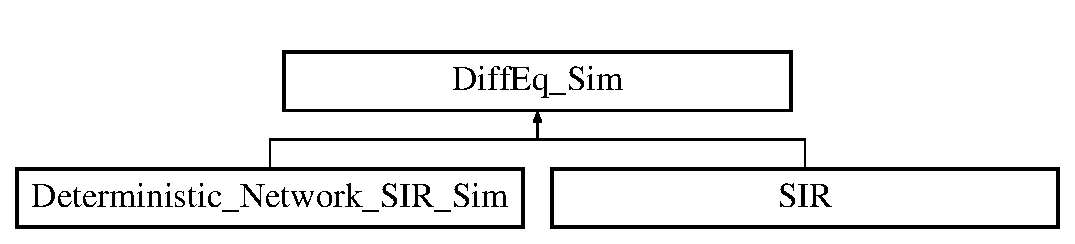
\includegraphics[height=2.000000cm]{classDiffEq__Sim}
\end{center}
\end{figure}
\subsection*{Public Member Functions}
\begin{DoxyCompactItemize}
\item 
\hypertarget{classDiffEq__Sim_a1bc98d13679395c4e9bb4a3e7e3d2722}{}void {\bfseries print\+Y} ()\label{classDiffEq__Sim_a1bc98d13679395c4e9bb4a3e7e3d2722}

\item 
\hypertarget{classDiffEq__Sim_aaae80a9a49cc714ae981d4122955f124}{}vector$<$ double $>$ {\bfseries get\+\_\+state} ()\label{classDiffEq__Sim_aaae80a9a49cc714ae981d4122955f124}

\item 
\hypertarget{classDiffEq__Sim_ade2acaa00bb9ee6d3ef84ae880cab290}{}double {\bfseries get\+\_\+time} ()\label{classDiffEq__Sim_ade2acaa00bb9ee6d3ef84ae880cab290}

\item 
\hypertarget{classDiffEq__Sim_aa5f364b0f3d90d833f390e155473b1ea}{}virtual void {\bfseries initialize} ()\label{classDiffEq__Sim_aa5f364b0f3d90d833f390e155473b1ea}

\item 
\hypertarget{classDiffEq__Sim_a77f15d45811b240771421ccb9e2dc1aa}{}virtual void {\bfseries derivative} (const double y\mbox{[}$\,$\mbox{]}, double dydt\mbox{[}$\,$\mbox{]})\label{classDiffEq__Sim_a77f15d45811b240771421ccb9e2dc1aa}

\item 
\hypertarget{classDiffEq__Sim_a6ba394082d829dfb5cdb2a98ac370169}{}int {\bfseries run\+\_\+simulation} ()\label{classDiffEq__Sim_a6ba394082d829dfb5cdb2a98ac370169}

\item 
\hypertarget{classDiffEq__Sim_a6812a26bfdcd0559f2e0a473ffb611c9}{}int {\bfseries step\+\_\+simulation} (double stepsize)\label{classDiffEq__Sim_a6812a26bfdcd0559f2e0a473ffb611c9}

\end{DoxyCompactItemize}
\subsection*{Static Public Member Functions}
\begin{DoxyCompactItemize}
\item 
\hypertarget{classDiffEq__Sim_a5eb1630bf8e5e80a40d44a006ae6c6bf}{}static int {\bfseries function} (double t, double const y\mbox{[}$\,$\mbox{]}, double dydt\mbox{[}$\,$\mbox{]}, void $\ast$params)\label{classDiffEq__Sim_a5eb1630bf8e5e80a40d44a006ae6c6bf}

\end{DoxyCompactItemize}
\subsection*{Public Attributes}
\begin{DoxyCompactItemize}
\item 
\hypertarget{classDiffEq__Sim_ace3d849259ca643078e87c2b8aaf6eb6}{}int {\bfseries nbins}\label{classDiffEq__Sim_ace3d849259ca643078e87c2b8aaf6eb6}

\item 
\hypertarget{classDiffEq__Sim_a67f5c9d51402d1ff94f3f9bd7f021475}{}double $\ast$ {\bfseries y}\label{classDiffEq__Sim_a67f5c9d51402d1ff94f3f9bd7f021475}

\end{DoxyCompactItemize}


The documentation for this class was generated from the following file\+:\begin{DoxyCompactItemize}
\item 
Diff\+Eq\+\_\+\+Sim.\+h\end{DoxyCompactItemize}

\hypertarget{classEdge}{}\section{Edge Class Reference}
\label{classEdge}\index{Edge@{Edge}}
\subsection*{Public Member Functions}
\begin{DoxyCompactItemize}
\item 
\hypertarget{classEdge_ac26d126cbd26713041dba5e28ea509b4}{}void {\bfseries delete\+\_\+edge} ()\label{classEdge_ac26d126cbd26713041dba5e28ea509b4}

\item 
\hypertarget{classEdge_ac544315709bb6180fbf626b7f0824fb5}{}void {\bfseries disconnect\+\_\+nodes} ()\label{classEdge_ac544315709bb6180fbf626b7f0824fb5}

\item 
\hypertarget{classEdge_a41de688b688ed7b033c683d0edd70d6f}{}int {\bfseries get\+\_\+id} ()\label{classEdge_a41de688b688ed7b033c683d0edd70d6f}

\item 
\hypertarget{classEdge_a3b40969f1821c69ca88bcbe190d77fa8}{}double {\bfseries get\+\_\+cost} ()\label{classEdge_a3b40969f1821c69ca88bcbe190d77fa8}

\item 
\hypertarget{classEdge_a21c32209277b91c97adc0b7bf73fdfa2}{}\hyperlink{classNode}{Node} $\ast$ {\bfseries get\+\_\+start} ()\label{classEdge_a21c32209277b91c97adc0b7bf73fdfa2}

\item 
\hypertarget{classEdge_a14b1b17cd5e63bc9986ddcd0318815f3}{}\hyperlink{classNode}{Node} $\ast$ {\bfseries get\+\_\+end} ()\label{classEdge_a14b1b17cd5e63bc9986ddcd0318815f3}

\item 
\hypertarget{classEdge_ad0d741fb5da9a6057f938a2d2cef7e8a}{}\hyperlink{classNetwork}{Network} $\ast$ {\bfseries get\+\_\+network} ()\label{classEdge_ad0d741fb5da9a6057f938a2d2cef7e8a}

\item 
\hypertarget{classEdge_af69eeda73987ab72d483cd95ad830cde}{}void {\bfseries set\+\_\+cost} (double c)\label{classEdge_af69eeda73987ab72d483cd95ad830cde}

\item 
\hypertarget{classEdge_aee63d265ded0609b41a3d5b84756c1ac}{}\hyperlink{classEdge}{Edge} $\ast$ {\bfseries get\+\_\+complement} ()\label{classEdge_aee63d265ded0609b41a3d5b84756c1ac}

\item 
\hypertarget{classEdge_ac6c6b1f954539af5673cbf711b211f19}{}void {\bfseries swap\+\_\+ends} (\hyperlink{classEdge}{Edge} $\ast$other\+\_\+edge)\label{classEdge_ac6c6b1f954539af5673cbf711b211f19}

\item 
\hypertarget{classEdge_a64c4bf1950f8eedd36f6bb5dbfdbc46f}{}void {\bfseries break\+\_\+end} ()\label{classEdge_a64c4bf1950f8eedd36f6bb5dbfdbc46f}

\item 
\hypertarget{classEdge_ad13aa9622d299c757a2a5d743b8a7018}{}void {\bfseries define\+\_\+end} (\hyperlink{classNode}{Node} $\ast$end\+\_\+node)\label{classEdge_ad13aa9622d299c757a2a5d743b8a7018}

\item 
\hypertarget{classEdge_a2c415df14bf24f20ce80738c140305e3}{}bool {\bfseries is\+\_\+stub} ()\label{classEdge_a2c415df14bf24f20ce80738c140305e3}

\item 
\hypertarget{classEdge_a9e86a5ffac43a72ca5f6b547f8a3fd61}{}bool {\bfseries operator==} (const \hyperlink{classEdge}{Edge} \&e2)\label{classEdge_a9e86a5ffac43a72ca5f6b547f8a3fd61}

\item 
\hypertarget{classEdge_a3f8c785f1c9873d7293bb31367b5611e}{}void {\bfseries dumper} ()\label{classEdge_a3f8c785f1c9873d7293bb31367b5611e}

\end{DoxyCompactItemize}
\subsection*{Friends}
\begin{DoxyCompactItemize}
\item 
\hypertarget{classEdge_a88b59289ffd793fecd040d32e397b1e9}{}class {\bfseries Network}\label{classEdge_a88b59289ffd793fecd040d32e397b1e9}

\item 
\hypertarget{classEdge_a6db9d28bd448a131448276ee03de1e6d}{}class {\bfseries Node}\label{classEdge_a6db9d28bd448a131448276ee03de1e6d}

\item 
\hypertarget{classEdge_a5a98f933c06debc7299f4e1086ab243d}{}ostream \& {\bfseries operator$<$$<$} (ostream \&out, \hyperlink{classEdge}{Edge} $\ast$edge)\label{classEdge_a5a98f933c06debc7299f4e1086ab243d}

\end{DoxyCompactItemize}


The documentation for this class was generated from the following files\+:\begin{DoxyCompactItemize}
\item 
Network.\+h\item 
Network.\+cpp\end{DoxyCompactItemize}

\hypertarget{classEvent}{}\section{Event Class Reference}
\label{classEvent}\index{Event@{Event}}
\subsection*{Public Member Functions}
\begin{DoxyCompactItemize}
\item 
\hypertarget{classEvent_abeb3fb64e44dec06fdb3e7278e0e045b}{}{\bfseries Event} (const \hyperlink{classEvent}{Event} \&o)\label{classEvent_abeb3fb64e44dec06fdb3e7278e0e045b}

\item 
\hypertarget{classEvent_a38585eb974c27a791695c2ae07680093}{}{\bfseries Event} (\hyperlink{classNode}{Node} $\ast$sink, int t, \hyperlink{classNode}{Node} $\ast$source)\label{classEvent_a38585eb974c27a791695c2ae07680093}

\item 
\hypertarget{classEvent_aba08af7e151431c376426ea6ad83ac76}{}\hyperlink{classEvent}{Event} \& {\bfseries operator=} (const \hyperlink{classEvent}{Event} \&o)\label{classEvent_aba08af7e151431c376426ea6ad83ac76}

\item 
\hypertarget{classEvent_abeb3fb64e44dec06fdb3e7278e0e045b}{}{\bfseries Event} (const \hyperlink{classEvent}{Event} \&o)\label{classEvent_abeb3fb64e44dec06fdb3e7278e0e045b}

\item 
\hypertarget{classEvent_aa1f26c73da20fa23029dbe6149220b29}{}{\bfseries Event} (double t, char e)\label{classEvent_aa1f26c73da20fa23029dbe6149220b29}

\item 
\hypertarget{classEvent_aba08af7e151431c376426ea6ad83ac76}{}\hyperlink{classEvent}{Event} \& {\bfseries operator=} (const \hyperlink{classEvent}{Event} \&o)\label{classEvent_aba08af7e151431c376426ea6ad83ac76}

\item 
\hypertarget{classEvent_abeb3fb64e44dec06fdb3e7278e0e045b}{}{\bfseries Event} (const \hyperlink{classEvent}{Event} \&o)\label{classEvent_abeb3fb64e44dec06fdb3e7278e0e045b}

\item 
\hypertarget{classEvent_a70b960ee98abf840b1d8016b60102d53}{}{\bfseries Event} (double t, char e, \hyperlink{classNode}{Node} $\ast$n)\label{classEvent_a70b960ee98abf840b1d8016b60102d53}

\item 
\hypertarget{classEvent_aba08af7e151431c376426ea6ad83ac76}{}\hyperlink{classEvent}{Event} \& {\bfseries operator=} (const \hyperlink{classEvent}{Event} \&o)\label{classEvent_aba08af7e151431c376426ea6ad83ac76}

\end{DoxyCompactItemize}
\subsection*{Public Attributes}
\begin{DoxyCompactItemize}
\item 
\hypertarget{classEvent_a3fe803b2b6c7bd89e27da7bb9780654a}{}\hyperlink{classNode}{Node} $\ast$ {\bfseries sink\+\_\+node}\label{classEvent_a3fe803b2b6c7bd89e27da7bb9780654a}

\item 
\hypertarget{classEvent_a7cf2572f1124c9700c89ff9f01b311bf}{}int {\bfseries time}\label{classEvent_a7cf2572f1124c9700c89ff9f01b311bf}

\item 
\hypertarget{classEvent_ad2be4bbe5fd7ea71576221bd21be6de0}{}\hyperlink{classNode}{Node} $\ast$ {\bfseries source\+\_\+node}\label{classEvent_ad2be4bbe5fd7ea71576221bd21be6de0}

\item 
\hypertarget{classEvent_a7cf2572f1124c9700c89ff9f01b311bf}{}double {\bfseries time}\label{classEvent_a7cf2572f1124c9700c89ff9f01b311bf}

\item 
\hypertarget{classEvent_a9bfb5a7398950cf1477e2dd365c93383}{}char {\bfseries type}\label{classEvent_a9bfb5a7398950cf1477e2dd365c93383}

\item 
\hypertarget{classEvent_abe1fedc4d0a92195dc9184183c99477a}{}\hyperlink{classNode}{Node} $\ast$ {\bfseries node}\label{classEvent_abe1fedc4d0a92195dc9184183c99477a}

\end{DoxyCompactItemize}


The documentation for this class was generated from the following files\+:\begin{DoxyCompactItemize}
\item 
Chain\+Binomial\+\_\+\+Sim.\+h\item 
Gillespie\+\_\+\+Mass\+Action\+\_\+\+Sim.\+h\item 
Gillespie\+\_\+\+Network\+\_\+\+S\+E\+I\+R\+S\+\_\+\+Sim.\+h\end{DoxyCompactItemize}

\hypertarget{classGillespie__MassAction__Sim}{}\section{Gillespie\+\_\+\+Mass\+Action\+\_\+\+Sim Class Reference}
\label{classGillespie__MassAction__Sim}\index{Gillespie\+\_\+\+Mass\+Action\+\_\+\+Sim@{Gillespie\+\_\+\+Mass\+Action\+\_\+\+Sim}}
\subsection*{Public Member Functions}
\begin{DoxyCompactItemize}
\item 
\hypertarget{classGillespie__MassAction__Sim_a9b4b53ea5569ec52d0e23dc2f7884cbe}{}{\bfseries Gillespie\+\_\+\+Mass\+Action\+\_\+\+Sim} (int n, double gamma, double beta)\label{classGillespie__MassAction__Sim_a9b4b53ea5569ec52d0e23dc2f7884cbe}

\item 
\hypertarget{classGillespie__MassAction__Sim_a6b570cc02daca342745fb1611aea90c9}{}void {\bfseries run\+\_\+simulation} ()\label{classGillespie__MassAction__Sim_a6b570cc02daca342745fb1611aea90c9}

\item 
\hypertarget{classGillespie__MassAction__Sim_a61d7cca8bfcaf0d97d03e4f4e8b35fc7}{}int {\bfseries epidemic\+\_\+size} ()\label{classGillespie__MassAction__Sim_a61d7cca8bfcaf0d97d03e4f4e8b35fc7}

\item 
\hypertarget{classGillespie__MassAction__Sim_a77c0557feada66744e3f11d941d90562}{}int {\bfseries reset} ()\label{classGillespie__MassAction__Sim_a77c0557feada66744e3f11d941d90562}

\item 
\hypertarget{classGillespie__MassAction__Sim_a41293b67dfb394ec78d26af72d34a49c}{}void {\bfseries rand\+\_\+infect} (int k)\label{classGillespie__MassAction__Sim_a41293b67dfb394ec78d26af72d34a49c}

\item 
\hypertarget{classGillespie__MassAction__Sim_ad043112abcf8ba09f3a5704acf38909b}{}void {\bfseries infect} ()\label{classGillespie__MassAction__Sim_ad043112abcf8ba09f3a5704acf38909b}

\item 
\hypertarget{classGillespie__MassAction__Sim_ac457e50469f3152894119b160b9b7986}{}bool {\bfseries is\+\_\+susceptible} (int x)\label{classGillespie__MassAction__Sim_ac457e50469f3152894119b160b9b7986}

\item 
\hypertarget{classGillespie__MassAction__Sim_aa0dcbe9596ee241c0821d1d138d3650d}{}int {\bfseries next\+\_\+event} ()\label{classGillespie__MassAction__Sim_aa0dcbe9596ee241c0821d1d138d3650d}

\item 
\hypertarget{classGillespie__MassAction__Sim_ad2dc4d3125dfa1e3c4f9a752b6a7f368}{}void {\bfseries add\+\_\+event} (double time, char type)\label{classGillespie__MassAction__Sim_ad2dc4d3125dfa1e3c4f9a752b6a7f368}

\end{DoxyCompactItemize}
\subsection*{Public Attributes}
\begin{DoxyCompactItemize}
\item 
\hypertarget{classGillespie__MassAction__Sim_adccdc2bfebe0292d126e45dfc6483714}{}int {\bfseries N}\label{classGillespie__MassAction__Sim_adccdc2bfebe0292d126e45dfc6483714}

\item 
\hypertarget{classGillespie__MassAction__Sim_a559d55e39e19391925dca421def8671e}{}double {\bfseries G\+A\+M\+M\+A}\label{classGillespie__MassAction__Sim_a559d55e39e19391925dca421def8671e}

\item 
\hypertarget{classGillespie__MassAction__Sim_a3b757a10891e669bc4eedb85464d6198}{}double {\bfseries B\+E\+T\+A}\label{classGillespie__MassAction__Sim_a3b757a10891e669bc4eedb85464d6198}

\item 
\hypertarget{classGillespie__MassAction__Sim_abf5bebde787931664d87e0068ff58416}{}priority\+\_\+queue$<$ \hyperlink{classEvent}{Event}, vector$<$ \hyperlink{classEvent}{Event} $>$, \hyperlink{classcompTime}{comp\+Time} $>$ {\bfseries Event\+Q}\label{classGillespie__MassAction__Sim_abf5bebde787931664d87e0068ff58416}

\item 
\hypertarget{classGillespie__MassAction__Sim_ab87320968791e1161a69c11a165d677d}{}vector$<$ int $>$ {\bfseries Compartments}\label{classGillespie__MassAction__Sim_ab87320968791e1161a69c11a165d677d}

\item 
\hypertarget{classGillespie__MassAction__Sim_aa47aeaba7d1f7809f4e67d8e4cbf76cb}{}double {\bfseries Now}\label{classGillespie__MassAction__Sim_aa47aeaba7d1f7809f4e67d8e4cbf76cb}

\item 
\hypertarget{classGillespie__MassAction__Sim_aee206f3e71c6b045e7ae80f0a1a4c57c}{}\hyperlink{classMTRand}{M\+T\+Rand} {\bfseries mtrand}\label{classGillespie__MassAction__Sim_aee206f3e71c6b045e7ae80f0a1a4c57c}

\end{DoxyCompactItemize}


The documentation for this class was generated from the following file\+:\begin{DoxyCompactItemize}
\item 
Gillespie\+\_\+\+Mass\+Action\+\_\+\+Sim.\+h\end{DoxyCompactItemize}

\hypertarget{classGillespie__Network__SEIRS__Sim}{}\section{Gillespie\+\_\+\+Network\+\_\+\+S\+E\+I\+R\+S\+\_\+\+Sim Class Reference}
\label{classGillespie__Network__SEIRS__Sim}\index{Gillespie\+\_\+\+Network\+\_\+\+S\+E\+I\+R\+S\+\_\+\+Sim@{Gillespie\+\_\+\+Network\+\_\+\+S\+E\+I\+R\+S\+\_\+\+Sim}}
\subsection*{Public Types}
\begin{DoxyCompactItemize}
\item 
\hypertarget{classGillespie__Network__SEIRS__Sim_abe4374e74f8a8693b420b1cd2eaeadfe}{}enum {\bfseries state\+Type} \{ \\*
{\bfseries S\+U\+S\+C\+E\+P\+T\+I\+B\+L\+E}, 
{\bfseries E\+X\+P\+O\+S\+E\+D}, 
{\bfseries I\+N\+F\+E\+C\+T\+I\+O\+U\+S}, 
{\bfseries R\+E\+S\+I\+S\+T\+A\+N\+T}, 
\\*
{\bfseries S\+T\+A\+T\+E\+\_\+\+S\+I\+Z\+E}
 \}\label{classGillespie__Network__SEIRS__Sim_abe4374e74f8a8693b420b1cd2eaeadfe}

\end{DoxyCompactItemize}
\subsection*{Public Member Functions}
\begin{DoxyCompactItemize}
\item 
\hypertarget{classGillespie__Network__SEIRS__Sim_af3ce0634c2db7ec0e52df194862d3c54}{}{\bfseries Gillespie\+\_\+\+Network\+\_\+\+S\+E\+I\+R\+S\+\_\+\+Sim} (\hyperlink{classNetwork}{Network} $\ast$net, double m, double b, double g, double im\+\_\+dur)\label{classGillespie__Network__SEIRS__Sim_af3ce0634c2db7ec0e52df194862d3c54}

\item 
\hypertarget{classGillespie__Network__SEIRS__Sim_ad40e3f247461baff81b5d4a09c50d1b5}{}void {\bfseries run\+\_\+simulation} (double duration)\label{classGillespie__Network__SEIRS__Sim_ad40e3f247461baff81b5d4a09c50d1b5}

\item 
\hypertarget{classGillespie__Network__SEIRS__Sim_a222828bfc04960db72c3e0c70d092c23}{}int {\bfseries current\+\_\+epidemic\+\_\+size} ()\label{classGillespie__Network__SEIRS__Sim_a222828bfc04960db72c3e0c70d092c23}

\item 
\hypertarget{classGillespie__Network__SEIRS__Sim_a61a0e4c7bdd2f4bbea0c8d243b451b0b}{}int {\bfseries reset} ()\label{classGillespie__Network__SEIRS__Sim_a61a0e4c7bdd2f4bbea0c8d243b451b0b}

\item 
\hypertarget{classGillespie__Network__SEIRS__Sim_a96af62a8a574e29b4f5984bbfbaa2887}{}vector$<$ \hyperlink{classNode}{Node} $\ast$ $>$ {\bfseries rand\+\_\+choose\+\_\+nodes} (int n)\label{classGillespie__Network__SEIRS__Sim_a96af62a8a574e29b4f5984bbfbaa2887}

\item 
\hypertarget{classGillespie__Network__SEIRS__Sim_a6aa0b3cd23a36e76c591d7395e428a92}{}void {\bfseries rand\+\_\+infect} (int n)\label{classGillespie__Network__SEIRS__Sim_a6aa0b3cd23a36e76c591d7395e428a92}

\item 
\hypertarget{classGillespie__Network__SEIRS__Sim_abae7c7a901f40ab3047a805fe7f91e4a}{}void {\bfseries infect} (\hyperlink{classNode}{Node} $\ast$node)\label{classGillespie__Network__SEIRS__Sim_abae7c7a901f40ab3047a805fe7f91e4a}

\item 
\hypertarget{classGillespie__Network__SEIRS__Sim_a3e1987e0ca831efafbc4cd7b470675f7}{}int {\bfseries next\+\_\+event} ()\label{classGillespie__Network__SEIRS__Sim_a3e1987e0ca831efafbc4cd7b470675f7}

\item 
\hypertarget{classGillespie__Network__SEIRS__Sim_a0b75c947ffb7646dfd43d7d2ee4dbad9}{}void {\bfseries add\+\_\+event} (double time, char type, \hyperlink{classNode}{Node} $\ast$node)\label{classGillespie__Network__SEIRS__Sim_a0b75c947ffb7646dfd43d7d2ee4dbad9}

\end{DoxyCompactItemize}
\subsection*{Public Attributes}
\begin{DoxyCompactItemize}
\item 
\hypertarget{classGillespie__Network__SEIRS__Sim_a3193fb9bf6b3dd896d72bdfcf04e4d42}{}\hyperlink{classNetwork}{Network} $\ast$ {\bfseries network}\label{classGillespie__Network__SEIRS__Sim_a3193fb9bf6b3dd896d72bdfcf04e4d42}

\item 
\hypertarget{classGillespie__Network__SEIRS__Sim_a04a4ebce166d5fe4db9b0682c4be6dcd}{}double {\bfseries mu}\label{classGillespie__Network__SEIRS__Sim_a04a4ebce166d5fe4db9b0682c4be6dcd}

\item 
\hypertarget{classGillespie__Network__SEIRS__Sim_a44df052180f79b45b03bc2e62235223e}{}double {\bfseries beta}\label{classGillespie__Network__SEIRS__Sim_a44df052180f79b45b03bc2e62235223e}

\item 
\hypertarget{classGillespie__Network__SEIRS__Sim_ae82ddeca49ef108857160ada93e2ec0a}{}double {\bfseries gamma}\label{classGillespie__Network__SEIRS__Sim_ae82ddeca49ef108857160ada93e2ec0a}

\item 
\hypertarget{classGillespie__Network__SEIRS__Sim_a24c4c1e7175470953a16b31094cbf732}{}double {\bfseries immunity\+\_\+duration}\label{classGillespie__Network__SEIRS__Sim_a24c4c1e7175470953a16b31094cbf732}

\item 
\hypertarget{classGillespie__Network__SEIRS__Sim_a15c255bee7c7ca340cf87df69f2566c4}{}priority\+\_\+queue$<$ \hyperlink{classEvent}{Event}, vector$<$ \hyperlink{classEvent}{Event} $>$, \hyperlink{classcompTime}{comp\+Time} $>$ {\bfseries Event\+Q}\label{classGillespie__Network__SEIRS__Sim_a15c255bee7c7ca340cf87df69f2566c4}

\item 
\hypertarget{classGillespie__Network__SEIRS__Sim_a8517dadca41d398109c7750fd9235570}{}vector$<$ int $>$ {\bfseries state\+\_\+counts}\label{classGillespie__Network__SEIRS__Sim_a8517dadca41d398109c7750fd9235570}

\item 
\hypertarget{classGillespie__Network__SEIRS__Sim_a919dd648216a95ded448aa21afda9b39}{}double {\bfseries Now}\label{classGillespie__Network__SEIRS__Sim_a919dd648216a95ded448aa21afda9b39}

\item 
\hypertarget{classGillespie__Network__SEIRS__Sim_a62f25b5c1c5a66b983f62c37f4bd0753}{}\hyperlink{classMTRand}{M\+T\+Rand} {\bfseries mtrand}\label{classGillespie__Network__SEIRS__Sim_a62f25b5c1c5a66b983f62c37f4bd0753}

\end{DoxyCompactItemize}


The documentation for this class was generated from the following file\+:\begin{DoxyCompactItemize}
\item 
Gillespie\+\_\+\+Network\+\_\+\+S\+E\+I\+R\+S\+\_\+\+Sim.\+h\end{DoxyCompactItemize}

\hypertarget{classIntervention}{}\section{Intervention Class Reference}
\label{classIntervention}\index{Intervention@{Intervention}}


The documentation for this class was generated from the following file\+:\begin{DoxyCompactItemize}
\item 
Intervention.\+h\end{DoxyCompactItemize}

\hypertarget{classMTRand}{}\section{M\+T\+Rand Class Reference}
\label{classMTRand}\index{M\+T\+Rand@{M\+T\+Rand}}
\subsection*{Public Types}
\begin{DoxyCompactItemize}
\item 
\hypertarget{classMTRand_ab8fea37d16b55e1a0fe06149e325f1b6}{}enum \{ {\bfseries N} = 624
 \}\label{classMTRand_ab8fea37d16b55e1a0fe06149e325f1b6}

\item 
\hypertarget{classMTRand_a7d9f4f1783a4e45f7834dd5174dfc2a1}{}enum \{ {\bfseries S\+A\+V\+E} = N + 1
 \}\label{classMTRand_a7d9f4f1783a4e45f7834dd5174dfc2a1}

\item 
\hypertarget{classMTRand_a45478edf9e24dcd2a5164bac3889d6a2}{}typedef unsigned long {\bfseries uint32}\label{classMTRand_a45478edf9e24dcd2a5164bac3889d6a2}

\end{DoxyCompactItemize}
\subsection*{Public Member Functions}
\begin{DoxyCompactItemize}
\item 
\hypertarget{classMTRand_ab4f392e44228a583b7b1a3f036fb2fd0}{}{\bfseries M\+T\+Rand} (const uint32 \&one\+Seed)\label{classMTRand_ab4f392e44228a583b7b1a3f036fb2fd0}

\item 
\hypertarget{classMTRand_a380e79e0192b46426abcefa6e2dd082e}{}{\bfseries M\+T\+Rand} (uint32 $\ast$const big\+Seed, uint32 const seed\+Length=N)\label{classMTRand_a380e79e0192b46426abcefa6e2dd082e}

\item 
\hypertarget{classMTRand_a76d129a2d850c24ff4a0613f299cf3a5}{}double {\bfseries rand} ()\label{classMTRand_a76d129a2d850c24ff4a0613f299cf3a5}

\item 
\hypertarget{classMTRand_a7a47382fb7b19ae1f330691735dc800b}{}double {\bfseries rand} (const double \&n)\label{classMTRand_a7a47382fb7b19ae1f330691735dc800b}

\item 
\hypertarget{classMTRand_afd05e468983b3a3d66ce0f403bd666af}{}double {\bfseries rand\+Exc} ()\label{classMTRand_afd05e468983b3a3d66ce0f403bd666af}

\item 
\hypertarget{classMTRand_a2955abdb96e6cab97e50ac755d48dad1}{}double {\bfseries rand\+Exc} (const double \&n)\label{classMTRand_a2955abdb96e6cab97e50ac755d48dad1}

\item 
\hypertarget{classMTRand_a4d3a475aa72fe6d1a6d7d9e16d6a732e}{}double {\bfseries rand\+Dbl\+Exc} ()\label{classMTRand_a4d3a475aa72fe6d1a6d7d9e16d6a732e}

\item 
\hypertarget{classMTRand_a587c90f52c35fa2bf05d34791dd5457e}{}double {\bfseries rand\+Dbl\+Exc} (const double \&n)\label{classMTRand_a587c90f52c35fa2bf05d34791dd5457e}

\item 
\hypertarget{classMTRand_ad1008efd4fe0e8aae30459c2c58cfe35}{}uint32 {\bfseries rand\+Int} ()\label{classMTRand_ad1008efd4fe0e8aae30459c2c58cfe35}

\item 
\hypertarget{classMTRand_a18ea21f615df06c9359c34d2eba6f252}{}uint32 {\bfseries rand\+Int} (const uint32 \&n)\label{classMTRand_a18ea21f615df06c9359c34d2eba6f252}

\item 
\hypertarget{classMTRand_abbb87a08d622d58fdee0eea4cb5471a0}{}double {\bfseries operator()} ()\label{classMTRand_abbb87a08d622d58fdee0eea4cb5471a0}

\item 
\hypertarget{classMTRand_a15f4daf79febbe4ff43c3e6ce2c4fcbe}{}double {\bfseries rand53} ()\label{classMTRand_a15f4daf79febbe4ff43c3e6ce2c4fcbe}

\item 
\hypertarget{classMTRand_a410775bb18f32161932b11f61f0fbd2c}{}double {\bfseries rand\+Norm} (const double \&mean=0.\+0, const double \&std\+\_\+dev=1.\+0)\label{classMTRand_a410775bb18f32161932b11f61f0fbd2c}

\item 
\hypertarget{classMTRand_a1e21a79e0a30225fffe924229e34a923}{}void {\bfseries seed} (const uint32 one\+Seed)\label{classMTRand_a1e21a79e0a30225fffe924229e34a923}

\item 
\hypertarget{classMTRand_a5758103776b131e8ea46b6dc1b9fb267}{}void {\bfseries seed} (uint32 $\ast$const big\+Seed, const uint32 seed\+Length=N)\label{classMTRand_a5758103776b131e8ea46b6dc1b9fb267}

\item 
\hypertarget{classMTRand_ad88ea3363d55bafb62826bbd130279c2}{}void {\bfseries seed} ()\label{classMTRand_ad88ea3363d55bafb62826bbd130279c2}

\item 
\hypertarget{classMTRand_ad60e0f3f5c90baab75b74f9a2ccae871}{}void {\bfseries save} (uint32 $\ast$save\+Array) const \label{classMTRand_ad60e0f3f5c90baab75b74f9a2ccae871}

\item 
\hypertarget{classMTRand_a8302e9a8cd16d8dfc536a85bf2f68be0}{}void {\bfseries load} (uint32 $\ast$const load\+Array)\label{classMTRand_a8302e9a8cd16d8dfc536a85bf2f68be0}

\end{DoxyCompactItemize}
\subsection*{Protected Types}
\begin{DoxyCompactItemize}
\item 
\hypertarget{classMTRand_a10c3437be98225f5b0beee1ed8c033c8}{}enum \{ {\bfseries M} = 397
 \}\label{classMTRand_a10c3437be98225f5b0beee1ed8c033c8}

\end{DoxyCompactItemize}
\subsection*{Protected Member Functions}
\begin{DoxyCompactItemize}
\item 
\hypertarget{classMTRand_a9b9a20998f5c805af6301ce5c37dcfc3}{}void {\bfseries initialize} (const uint32 one\+Seed)\label{classMTRand_a9b9a20998f5c805af6301ce5c37dcfc3}

\item 
\hypertarget{classMTRand_a1d5fcb69d83f4d2fd653883c8352f86c}{}void {\bfseries reload} ()\label{classMTRand_a1d5fcb69d83f4d2fd653883c8352f86c}

\item 
\hypertarget{classMTRand_a0f44969adf5a2991ad73b8bc4608c5c7}{}uint32 {\bfseries hi\+Bit} (const uint32 \&u) const \label{classMTRand_a0f44969adf5a2991ad73b8bc4608c5c7}

\item 
\hypertarget{classMTRand_a440ff2c31889aa6dde5babbe862a9e14}{}uint32 {\bfseries lo\+Bit} (const uint32 \&u) const \label{classMTRand_a440ff2c31889aa6dde5babbe862a9e14}

\item 
\hypertarget{classMTRand_a9032b296e470bed53280a452e55203b7}{}uint32 {\bfseries lo\+Bits} (const uint32 \&u) const \label{classMTRand_a9032b296e470bed53280a452e55203b7}

\item 
\hypertarget{classMTRand_ae7eb1282079e30b0a4a526cb86f8c2a2}{}uint32 {\bfseries mix\+Bits} (const uint32 \&u, const uint32 \&v) const \label{classMTRand_ae7eb1282079e30b0a4a526cb86f8c2a2}

\item 
\hypertarget{classMTRand_af1219020248cb80b772d64e2b6151a9c}{}uint32 {\bfseries twist} (const uint32 \&m, const uint32 \&s0, const uint32 \&s1) const \label{classMTRand_af1219020248cb80b772d64e2b6151a9c}

\end{DoxyCompactItemize}
\subsection*{Static Protected Member Functions}
\begin{DoxyCompactItemize}
\item 
\hypertarget{classMTRand_a486885d03f38c844315d002e6312fa23}{}static uint32 {\bfseries hash} (time\+\_\+t t, clock\+\_\+t c)\label{classMTRand_a486885d03f38c844315d002e6312fa23}

\end{DoxyCompactItemize}
\subsection*{Protected Attributes}
\begin{DoxyCompactItemize}
\item 
\hypertarget{classMTRand_a2c87f537429bf0b0f6a452c22b9eebba}{}uint32 {\bfseries state} \mbox{[}N\mbox{]}\label{classMTRand_a2c87f537429bf0b0f6a452c22b9eebba}

\item 
\hypertarget{classMTRand_a2b80858137c88fe69d4d2bdc665bcf93}{}uint32 $\ast$ {\bfseries p\+Next}\label{classMTRand_a2b80858137c88fe69d4d2bdc665bcf93}

\item 
\hypertarget{classMTRand_a98eabf568c88f121e44f487397f32495}{}int {\bfseries left}\label{classMTRand_a98eabf568c88f121e44f487397f32495}

\end{DoxyCompactItemize}
\subsection*{Friends}
\begin{DoxyCompactItemize}
\item 
\hypertarget{classMTRand_a059061d50a1e54ee3067d4e1dbdd7c64}{}std\+::ostream \& {\bfseries operator$<$$<$} (std\+::ostream \&os, const \hyperlink{classMTRand}{M\+T\+Rand} \&mtrand)\label{classMTRand_a059061d50a1e54ee3067d4e1dbdd7c64}

\item 
\hypertarget{classMTRand_a45b02a702835a3be42171c5c2dc79b2d}{}std\+::istream \& {\bfseries operator$>$$>$} (std\+::istream \&is, \hyperlink{classMTRand}{M\+T\+Rand} \&mtrand)\label{classMTRand_a45b02a702835a3be42171c5c2dc79b2d}

\end{DoxyCompactItemize}


The documentation for this class was generated from the following file\+:\begin{DoxyCompactItemize}
\item 
Mersenne\+Twister.\+h\end{DoxyCompactItemize}

\hypertarget{classNetwork}{}\section{Network Class Reference}
\label{classNetwork}\index{Network@{Network}}
\subsection*{Public Types}
\begin{DoxyCompactItemize}
\item 
\hypertarget{classNetwork_a7e628548107e46864ae0c856bf5aaa9f}{}enum {\bfseries net\+Type} \{ {\bfseries Undirected} =0, 
{\bfseries Directed} =1
 \}\label{classNetwork_a7e628548107e46864ae0c856bf5aaa9f}

\item 
\hypertarget{classNetwork_a1743227a9ab62bdffe7eaf5e6826ca74}{}enum {\bfseries output\+Type} \{ {\bfseries Node\+Names} =0, 
{\bfseries Node\+I\+Ds} =1
 \}\label{classNetwork_a1743227a9ab62bdffe7eaf5e6826ca74}

\end{DoxyCompactItemize}
\subsection*{Public Member Functions}
\begin{DoxyCompactItemize}
\item 
\hypertarget{classNetwork_ae75eec96cb0933276170cd5b1a5d715e}{}{\bfseries Network} (string name, net\+Type directed)\label{classNetwork_ae75eec96cb0933276170cd5b1a5d715e}

\item 
\hypertarget{classNetwork_a8f7bc88d89cf3f52600b792bb9985010}{}{\bfseries Network} (const \hyperlink{classNetwork}{Network} \&net)\label{classNetwork_a8f7bc88d89cf3f52600b792bb9985010}

\item 
\hypertarget{classNetwork_a00a122e905f834927294533dd1e99788}{}\hyperlink{classNetwork}{Network} $\ast$ {\bfseries duplicate} ()\label{classNetwork_a00a122e905f834927294533dd1e99788}

\item 
\hypertarget{classNetwork_adb84b687ca9b3898ac7de910654dc6ed}{}bool {\bfseries operator==} (const \hyperlink{classNetwork}{Network} \&n2)\label{classNetwork_adb84b687ca9b3898ac7de910654dc6ed}

\item 
\hypertarget{classNetwork_af24aaed953f573bb2b19a1db78734fb0}{}int {\bfseries get\+\_\+id} ()\label{classNetwork_af24aaed953f573bb2b19a1db78734fb0}

\item 
\hypertarget{classNetwork_a37e0e9e2db034f6b549a9a0198cd9d75}{}string {\bfseries get\+\_\+name} ()\label{classNetwork_a37e0e9e2db034f6b549a9a0198cd9d75}

\item 
\hypertarget{classNetwork_a0da93244ee6aa2c51af37aa193481330}{}int {\bfseries size} ()\label{classNetwork_a0da93244ee6aa2c51af37aa193481330}

\item 
\hypertarget{classNetwork_afbf84b31a0cc3fa9d41411fae0afcb46}{}bool {\bfseries has\+\_\+unit\+\_\+edges} ()\label{classNetwork_afbf84b31a0cc3fa9d41411fae0afcb46}

\item 
\hypertarget{classNetwork_a5bc3e3d4a34b0a5d888c291c8946db75}{}bool {\bfseries is\+\_\+directed} ()\label{classNetwork_a5bc3e3d4a34b0a5d888c291c8946db75}

\item 
\hypertarget{classNetwork_a15b38693e92c7f62e3d6c7c8c1227499}{}\hyperlink{classMTRand}{M\+T\+Rand} $\ast$ {\bfseries get\+\_\+rng} ()\label{classNetwork_a15b38693e92c7f62e3d6c7c8c1227499}

\item 
\hypertarget{classNetwork_ace9c30eb87c661132f910fb1345afc48}{}vector$<$ \hyperlink{classNode}{Node} $\ast$ $>$ {\bfseries get\+\_\+nodes} ()\label{classNetwork_ace9c30eb87c661132f910fb1345afc48}

\item 
\hypertarget{classNetwork_a709ce39807cad7c87f13692d26c87274}{}\hyperlink{classNode}{Node} $\ast$ {\bfseries get\+\_\+node} (int node\+\_\+id)\label{classNetwork_a709ce39807cad7c87f13692d26c87274}

\item 
\hypertarget{classNetwork_aeabfba6ab4874667882749594de7dada}{}\hyperlink{classNode}{Node} $\ast$ {\bfseries get\+\_\+node\+\_\+by\+\_\+name} (string node\+\_\+name)\label{classNetwork_aeabfba6ab4874667882749594de7dada}

\item 
\hypertarget{classNetwork_ad9312ef8bc67d27066cfbebc8794e313}{}\hyperlink{classNode}{Node} $\ast$ {\bfseries get\+\_\+rand\+\_\+node} ()\label{classNetwork_ad9312ef8bc67d27066cfbebc8794e313}

\item 
\hypertarget{classNetwork_a7c009bf7dde31ee211045212f47b0710}{}vector$<$ \hyperlink{classEdge}{Edge} $\ast$ $>$ {\bfseries get\+\_\+edges} ()\label{classNetwork_a7c009bf7dde31ee211045212f47b0710}

\item 
\hypertarget{classNetwork_afd8a3ade922ecd10c333b5d3bb3621de}{}\hyperlink{classEdge}{Edge} $\ast$ {\bfseries get\+\_\+edge} (int id)\label{classNetwork_afd8a3ade922ecd10c333b5d3bb3621de}

\item 
\hypertarget{classNetwork_a99010c3efb17d60477fd48b2b667d783}{}vector$<$ state\+Type $>$ {\bfseries get\+\_\+node\+\_\+states} ()\label{classNetwork_a99010c3efb17d60477fd48b2b667d783}

\item 
\hypertarget{classNetwork_a4a3afc7f166ccaf84560740ca9a4caaa}{}void {\bfseries get\+\_\+bad\+\_\+edges} (vector$<$ \hyperlink{classEdge}{Edge} $\ast$ $>$ \&self\+\_\+loops, vector$<$ \hyperlink{classEdge}{Edge} $\ast$ $>$ \&multiedges)\label{classNetwork_a4a3afc7f166ccaf84560740ca9a4caaa}

\item 
\hypertarget{classNetwork_a2787d023f770195e241442cd5934ac6c}{}vector$<$ \hyperlink{classNode}{Node} $\ast$ $>$ {\bfseries get\+\_\+component} (\hyperlink{classNode}{Node} $\ast$node)\label{classNetwork_a2787d023f770195e241442cd5934ac6c}

\item 
\hypertarget{classNetwork_aaa803fd081ed5f24a38c981055fd459d}{}vector$<$ vector$<$ \hyperlink{classNode}{Node} $\ast$ $>$ $>$ {\bfseries get\+\_\+components} ()\label{classNetwork_aaa803fd081ed5f24a38c981055fd459d}

\item 
\hypertarget{classNetwork_aad3d529c979cefd275f1c72c51aedff8}{}vector$<$ \hyperlink{classNode}{Node} $\ast$ $>$ {\bfseries get\+\_\+biggest\+\_\+component} ()\label{classNetwork_aad3d529c979cefd275f1c72c51aedff8}

\item 
\hypertarget{classNetwork_aac7db1edc83f6ee1811545504d391944}{}bool {\bfseries topology\+\_\+altered} ()\label{classNetwork_aac7db1edc83f6ee1811545504d391944}

\item 
\hypertarget{classNetwork_a18f85b48490f70707eb0d3ecf3af3bb7}{}\hyperlink{classNode}{Node} $\ast$ {\bfseries add\+\_\+new\+\_\+node} ()\label{classNetwork_a18f85b48490f70707eb0d3ecf3af3bb7}

\item 
\hypertarget{classNetwork_a43c10781b1a8cd9d1d45631524619e12}{}void {\bfseries populate} (int n)\label{classNetwork_a43c10781b1a8cd9d1d45631524619e12}

\item 
\hypertarget{classNetwork_aaf0e1975514749d95d7e3baeb931c176}{}void {\bfseries add\+\_\+node} (\hyperlink{classNode}{Node} $\ast$node)\label{classNetwork_aaf0e1975514749d95d7e3baeb931c176}

\item 
\hypertarget{classNetwork_afa5ba9cc04dd16835794edc3a9069f73}{}void {\bfseries delete\+\_\+node} (\hyperlink{classNode}{Node} $\ast$node)\label{classNetwork_afa5ba9cc04dd16835794edc3a9069f73}

\item 
\hypertarget{classNetwork_a3b1aed2ba4355e1b6429afc43105632e}{}bool {\bfseries all\+\_\+to\+\_\+all\+\_\+coupling} ()\label{classNetwork_a3b1aed2ba4355e1b6429afc43105632e}

\item 
\hypertarget{classNetwork_a1bc00a48e15b686922ea929d2d9cfef9}{}bool {\bfseries erdos\+\_\+renyi} (double lambda)\label{classNetwork_a1bc00a48e15b686922ea929d2d9cfef9}

\item 
\hypertarget{classNetwork_aeb3c4bdf9689a323e124c05f7829798f}{}bool {\bfseries sparse\+\_\+random\+\_\+graph} (double lambda)\label{classNetwork_aeb3c4bdf9689a323e124c05f7829798f}

\item 
\hypertarget{classNetwork_ad43dcfdc9ae6eceba263345fcf89a8d2}{}bool {\bfseries fast\+\_\+random\+\_\+graph} (double lambda)\label{classNetwork_ad43dcfdc9ae6eceba263345fcf89a8d2}

\item 
\hypertarget{classNetwork_a669fa9b5563bfffafc0fa8e9a48eb867}{}bool {\bfseries ring\+\_\+lattice} (int N, int K)\label{classNetwork_a669fa9b5563bfffafc0fa8e9a48eb867}

\item 
\hypertarget{classNetwork_a04933d68710bb79fec7bd8e10ec19f9d}{}bool {\bfseries square\+\_\+lattice} (int R, int C, bool diag)\label{classNetwork_a04933d68710bb79fec7bd8e10ec19f9d}

\item 
\hypertarget{classNetwork_a29c5d2dd1efbc9f40c3a0e318e49036c}{}bool {\bfseries small\+\_\+world} (int N, int K, double beta)\label{classNetwork_a29c5d2dd1efbc9f40c3a0e318e49036c}

\item 
\hypertarget{classNetwork_abd6b9fe591b882fc716738fb612d89fa}{}bool {\bfseries rand\+\_\+connect\+\_\+poisson} (double lambda)\label{classNetwork_abd6b9fe591b882fc716738fb612d89fa}

\item 
\hypertarget{classNetwork_a414dde2a6bcd5f9cb45e5cab6452c852}{}bool {\bfseries rand\+\_\+connect\+\_\+powerlaw} (double alpha, double kappa)\label{classNetwork_a414dde2a6bcd5f9cb45e5cab6452c852}

\item 
\hypertarget{classNetwork_a068af8f9da7939151dbeedbef35af9d0}{}bool {\bfseries rand\+\_\+connect\+\_\+exponential} (double lambda)\label{classNetwork_a068af8f9da7939151dbeedbef35af9d0}

\item 
\hypertarget{classNetwork_af0dc0df3f919b35d6c5586c8cbc71634}{}bool {\bfseries rand\+\_\+connect\+\_\+user} (vector$<$ double $>$ dist)\label{classNetwork_af0dc0df3f919b35d6c5586c8cbc71634}

\item 
\hypertarget{classNetwork_a0ecaab9f51f811cdc1071b66d3e358b6}{}bool {\bfseries rand\+\_\+connect\+\_\+explicit} (vector$<$ int $>$ deg\+\_\+series)\label{classNetwork_a0ecaab9f51f811cdc1071b66d3e358b6}

\item 
\hypertarget{classNetwork_a3769c229ac52fb7c7aff373747a002b8}{}bool {\bfseries rand\+\_\+connect\+\_\+stubs} (vector$<$ \hyperlink{classEdge}{Edge} $\ast$ $>$ stubs)\label{classNetwork_a3769c229ac52fb7c7aff373747a002b8}

\item 
\hypertarget{classNetwork_abde72ca35cf99ff927385c8f7843490f}{}bool {\bfseries lose\+\_\+loops} ()\label{classNetwork_abde72ca35cf99ff927385c8f7843490f}

\item 
\hypertarget{classNetwork_af8886395b3c292a670c7ffed1610448e}{}void {\bfseries clear\+\_\+nodes} ()\label{classNetwork_af8886395b3c292a670c7ffed1610448e}

\item 
\hypertarget{classNetwork_a80e6909a2fcf656ae8f720920b7a721d}{}void {\bfseries clear\+\_\+edges} ()\label{classNetwork_a80e6909a2fcf656ae8f720920b7a721d}

\item 
\hypertarget{classNetwork_a1d655233d6f1e7e976eb72c28d7ffe02}{}void {\bfseries disconnect\+\_\+edges} ()\label{classNetwork_a1d655233d6f1e7e976eb72c28d7ffe02}

\item 
\hypertarget{classNetwork_aeae904a08d9d5e7f8b8735a06f0d96f9}{}bool {\bfseries shuffle\+\_\+edges} (double frac)\label{classNetwork_aeae904a08d9d5e7f8b8735a06f0d96f9}

\item 
\hypertarget{classNetwork_af00312d958665700967525224eaf3171}{}void {\bfseries set\+\_\+node\+\_\+states} (vector$<$ state\+Type $>$ \&states)\label{classNetwork_af00312d958665700967525224eaf3171}

\item 
\hypertarget{classNetwork_adabe89c6c5d79192e5149aab1c79686d}{}void {\bfseries initialize} (double mean\+\_\+coupling, double var\+\_\+coupling, double mean\+\_\+preference, double var\+\_\+preference, double mean\+\_\+initial\+\_\+state)\label{classNetwork_adabe89c6c5d79192e5149aab1c79686d}

\item 
\hypertarget{classNetwork_a5be5e3f143bc528d37c49e0406b7b039}{}void {\bfseries set\+\_\+topology\+\_\+altered} (bool flag)\label{classNetwork_a5be5e3f143bc528d37c49e0406b7b039}

\item 
\hypertarget{classNetwork_a7daffc01be38d41fb0bf8de762e12642}{}void {\bfseries read\+\_\+edgelist} (string filename, char sep= \textquotesingle{},\textquotesingle{})\label{classNetwork_a7daffc01be38d41fb0bf8de762e12642}

\item 
\hypertarget{classNetwork_a7955ccfdf8578129ff7d78b68b9b70e3}{}void {\bfseries write\+\_\+edgelist} (string filename, output\+Type names\+\_\+or\+\_\+ids, char sep= \textquotesingle{},\textquotesingle{})\label{classNetwork_a7955ccfdf8578129ff7d78b68b9b70e3}

\item 
\hypertarget{classNetwork_a715ff2af7d730dfbf6dcc7df6f1d5f1e}{}void {\bfseries graphviz} (string filename)\label{classNetwork_a715ff2af7d730dfbf6dcc7df6f1d5f1e}

\item 
\hypertarget{classNetwork_ad1a7e13122c4f9f57cf18c4209dfe36e}{}void {\bfseries dumper} ()\label{classNetwork_ad1a7e13122c4f9f57cf18c4209dfe36e}

\item 
\hypertarget{classNetwork_a4e178cc9e4b881720e87ee74079f3eca}{}bool {\bfseries gen\+\_\+deg\+\_\+series} (vector$<$ int $>$ \&deg\+\_\+series)\label{classNetwork_a4e178cc9e4b881720e87ee74079f3eca}

\item 
\hypertarget{classNetwork_af81e5b4d67998d298017ec9ec66484e2}{}vector$<$ state\+Type $>$ {\bfseries get\+\_\+states} ()\label{classNetwork_af81e5b4d67998d298017ec9ec66484e2}

\item 
\hypertarget{classNetwork_a1692dbef538bf487d16188a59b4e46a0}{}vector$<$ vector$<$ state\+Type $>$ $>$ {\bfseries get\+\_\+states\+\_\+by\+\_\+degree} ()\label{classNetwork_a1692dbef538bf487d16188a59b4e46a0}

\item 
\hypertarget{classNetwork_a5573ffefb3a8890ec33510268024c32f}{}double {\bfseries get\+\_\+coarse\+\_\+state} ()\label{classNetwork_a5573ffefb3a8890ec33510268024c32f}

\item 
\hypertarget{classNetwork_a4d400d268d537cbd00b1703a5ad74103}{}bool {\bfseries validate} ()\label{classNetwork_a4d400d268d537cbd00b1703a5ad74103}

\item 
\hypertarget{classNetwork_a8e72ffb8dcc1ea35bffbca3c1acb50d9}{}vector$<$ int $>$ {\bfseries get\+\_\+deg\+\_\+series} ()\label{classNetwork_a8e72ffb8dcc1ea35bffbca3c1acb50d9}

\item 
\hypertarget{classNetwork_a1472b8a33c27fccb2cd3b84062a6bb4b}{}vector$<$ int $>$ {\bfseries get\+\_\+deg\+\_\+dist} ()\label{classNetwork_a1472b8a33c27fccb2cd3b84062a6bb4b}

\item 
\hypertarget{classNetwork_a14841f262bd881614eb9311543fa0af7}{}vector$<$ double $>$ {\bfseries get\+\_\+gen\+\_\+deg\+\_\+dist} ()\label{classNetwork_a14841f262bd881614eb9311543fa0af7}

\item 
\hypertarget{classNetwork_aecc7b85001c902af1aa0a4b086fd0ed2}{}double {\bfseries mean\+\_\+deg} ()\label{classNetwork_aecc7b85001c902af1aa0a4b086fd0ed2}

\item 
\hypertarget{classNetwork_a436e1276adc9ba3fd7f7e6df05669694}{}map$<$ \hyperlink{classNode}{Node} $\ast$, int $>$ {\bfseries k\+\_\+shell\+\_\+decomposition} ()\label{classNetwork_a436e1276adc9ba3fd7f7e6df05669694}

\item 
\hypertarget{classNetwork_aea6f2b6662fb3894df7949ba44ff8b7c}{}double {\bfseries transitivity} ()\label{classNetwork_aea6f2b6662fb3894df7949ba44ff8b7c}

\item 
\hypertarget{classNetwork_a59d0553fe4819979e6bb432f2e4a2a99}{}double {\bfseries transitivity} (vector$<$ \hyperlink{classNode}{Node} $\ast$ $>$ node\+\_\+set)\label{classNetwork_a59d0553fe4819979e6bb432f2e4a2a99}

\item 
\hypertarget{classNetwork_a0668d8c063328bfe611f56c27509a8be}{}bool {\bfseries is\+\_\+weighted} ()\label{classNetwork_a0668d8c063328bfe611f56c27509a8be}

\item 
\hypertarget{classNetwork_a0a92d8f5afe94a16ed6446b6435959a5}{}double {\bfseries mean\+\_\+dist} (vector$<$ \hyperlink{classNode}{Node} $\ast$ $>$ node\+\_\+set)\label{classNetwork_a0a92d8f5afe94a16ed6446b6435959a5}

\item 
\hypertarget{classNetwork_a48d1feba1bd00925ef2b3b8710d7f237}{}void {\bfseries calculate\+\_\+distances} (vector$<$ \hyperlink{classNode}{Node} $\ast$ $>$ \&destinations, vector$<$ vector$<$ double $>$ $>$ \&distances)\label{classNetwork_a48d1feba1bd00925ef2b3b8710d7f237}

\item 
\hypertarget{classNetwork_a40116699c4df6117b9c24b877410520d}{}void {\bfseries print\+\_\+distances} (vector$<$ \hyperlink{classNode}{Node} $\ast$ $>$ \&full\+\_\+node\+\_\+set)\label{classNetwork_a40116699c4df6117b9c24b877410520d}

\item 
\hypertarget{classNetwork_a07a00fc58e7f7e0b63460c29084b8688}{}void {\bfseries stop\+\_\+processing} ()\label{classNetwork_a07a00fc58e7f7e0b63460c29084b8688}

\item 
\hypertarget{classNetwork_a4b96943d9095e3922741688add7ca818}{}void {\bfseries reset\+\_\+processing\+\_\+flag} ()\label{classNetwork_a4b96943d9095e3922741688add7ca818}

\end{DoxyCompactItemize}
\subsection*{Friends}
\begin{DoxyCompactItemize}
\item 
\hypertarget{classNetwork_a6db9d28bd448a131448276ee03de1e6d}{}class {\bfseries Node}\label{classNetwork_a6db9d28bd448a131448276ee03de1e6d}

\item 
\hypertarget{classNetwork_ad2c8ba04c9d9989ccbf3c5aba267a3d7}{}class {\bfseries Edge}\label{classNetwork_ad2c8ba04c9d9989ccbf3c5aba267a3d7}

\end{DoxyCompactItemize}


The documentation for this class was generated from the following files\+:\begin{DoxyCompactItemize}
\item 
Network.\+h\item 
Network.\+cpp\end{DoxyCompactItemize}

\hypertarget{classNode}{}\section{Node Class Reference}
\label{classNode}\index{Node@{Node}}
\subsection*{Public Member Functions}
\begin{DoxyCompactItemize}
\item 
\hypertarget{classNode_a84588c0426ecba3f272158e901a147f4}{}bool {\bfseries is\+\_\+stopped} ()\label{classNode_a84588c0426ecba3f272158e901a147f4}

\item 
\hypertarget{classNode_a91f1b8c208c71d40b99ee747422ded86}{}void {\bfseries delete\+\_\+node} ()\label{classNode_a91f1b8c208c71d40b99ee747422ded86}

\item 
\hypertarget{classNode_afb8137c4ef9bfb7f3bb5285897d766af}{}void {\bfseries set\+\_\+network} (\hyperlink{classNetwork}{Network} $\ast$network)\label{classNode_afb8137c4ef9bfb7f3bb5285897d766af}

\item 
\hypertarget{classNode_a0be494ea471ea887e4becbeb32def3e9}{}int {\bfseries get\+\_\+id} ()\label{classNode_a0be494ea471ea887e4becbeb32def3e9}

\item 
\hypertarget{classNode_a81e9f5e01dea4e47abf7a911b5bc5296}{}string {\bfseries get\+\_\+name} ()\label{classNode_a81e9f5e01dea4e47abf7a911b5bc5296}

\item 
\hypertarget{classNode_aa820f9bda2d2780f2249e1ead61cbc8c}{}\hyperlink{classNetwork}{Network} $\ast$ {\bfseries get\+\_\+network} ()\label{classNode_aa820f9bda2d2780f2249e1ead61cbc8c}

\item 
\hypertarget{classNode_ae5c6daf380dc280cf620d941e3d68f7b}{}vector$<$ \hyperlink{classEdge}{Edge} $\ast$ $>$ {\bfseries get\+\_\+edges\+\_\+in} ()\label{classNode_ae5c6daf380dc280cf620d941e3d68f7b}

\item 
\hypertarget{classNode_a2ea047846eeca09af1b6ce4b33794f31}{}vector$<$ \hyperlink{classEdge}{Edge} $\ast$ $>$ {\bfseries get\+\_\+edges\+\_\+out} ()\label{classNode_a2ea047846eeca09af1b6ce4b33794f31}

\item 
\hypertarget{classNode_a3897d13b879221d499c6c2ec9b38b0f6}{}vector$<$ double $>$ {\bfseries get\+\_\+loc} ()\label{classNode_a3897d13b879221d499c6c2ec9b38b0f6}

\item 
\hypertarget{classNode_a181aa95b360895ddef089d101139e575}{}state\+Type {\bfseries get\+\_\+state} ()\label{classNode_a181aa95b360895ddef089d101139e575}

\item 
\hypertarget{classNode_a17942130651f990fe309dfcb07e36968}{}double {\bfseries get\+\_\+coupling} ()\label{classNode_a17942130651f990fe309dfcb07e36968}

\item 
\hypertarget{classNode_a70162b517042d6fc391179bceef4d889}{}double {\bfseries get\+\_\+preference} ()\label{classNode_a70162b517042d6fc391179bceef4d889}

\item 
\hypertarget{classNode_aa9c34bdb51c5ee84c2c5991b75ce458c}{}double {\bfseries get\+\_\+utility} ()\label{classNode_aa9c34bdb51c5ee84c2c5991b75ce458c}

\item 
\hypertarget{classNode_aa6f170ffb5f310911f8af75a1db93b3d}{}void {\bfseries set\+\_\+loc} (const vector$<$ double $>$ \&newloc)\label{classNode_aa6f170ffb5f310911f8af75a1db93b3d}

\item 
\hypertarget{classNode_a87ec83fad299cbedad57142a4e0e0d01}{}void {\bfseries set\+\_\+state} (state\+Type s)\label{classNode_a87ec83fad299cbedad57142a4e0e0d01}

\item 
\hypertarget{classNode_ac80c09e6bbfb596056f46aa0bc062dfb}{}void {\bfseries set\+\_\+coupling} (double c)\label{classNode_ac80c09e6bbfb596056f46aa0bc062dfb}

\item 
\hypertarget{classNode_adc2403ba1af5b94ef065026d483789c6}{}void {\bfseries set\+\_\+preference} (double p)\label{classNode_adc2403ba1af5b94ef065026d483789c6}

\item 
\hypertarget{classNode_ab75b1dbbb46825c3cb5329047cacb1a3}{}double {\bfseries mean\+\_\+min\+\_\+path} ()\label{classNode_ab75b1dbbb46825c3cb5329047cacb1a3}

\item 
\hypertarget{classNode_a989a2bec38b01c8048535fac84aa01ad}{}vector$<$ double $>$ {\bfseries min\+\_\+paths} (vector$<$ \hyperlink{classNode}{Node} $\ast$ $>$ \&node\+\_\+set)\label{classNode_a989a2bec38b01c8048535fac84aa01ad}

\item 
\hypertarget{classNode_a35610e36dabdf0ac0d31c858ba9dce76}{}void {\bfseries add\+\_\+stubs} (int deg)\label{classNode_a35610e36dabdf0ac0d31c858ba9dce76}

\item 
\hypertarget{classNode_ad82b8e548dbe9ac08da97d91cfcd5504}{}\hyperlink{classEdge}{Edge} $\ast$ {\bfseries get\+\_\+rand\+\_\+edge} ()\label{classNode_ad82b8e548dbe9ac08da97d91cfcd5504}

\item 
\hypertarget{classNode_a66879b4a454db6b9ae77eb6a2d00f838}{}vector$<$ \hyperlink{classNode}{Node} $\ast$ $>$ {\bfseries get\+\_\+neighbors} ()\label{classNode_a66879b4a454db6b9ae77eb6a2d00f838}

\item 
\hypertarget{classNode_aac4cc347fc2c7e0ab05e6d5238e11c92}{}double {\bfseries get\+\_\+neighbors\+\_\+state} ()\label{classNode_aac4cc347fc2c7e0ab05e6d5238e11c92}

\item 
\hypertarget{classNode_a71cb643a85948da88e39b93f7cfba11b}{}void {\bfseries update\+\_\+utility\+\_\+function} ()\label{classNode_a71cb643a85948da88e39b93f7cfba11b}

\item 
\hypertarget{classNode_a4350c87c78c07d38cac119ab37a84668}{}bool {\bfseries is\+\_\+neighbor} (\hyperlink{classNode}{Node} $\ast$node2)\label{classNode_a4350c87c78c07d38cac119ab37a84668}

\item 
\hypertarget{classNode_a1898c016e7fd43090b584ef82dbffe94}{}void {\bfseries connect\+\_\+to} (\hyperlink{classNode}{Node} $\ast$end)\label{classNode_a1898c016e7fd43090b584ef82dbffe94}

\item 
\hypertarget{classNode_afa26891f04784f67c2b43c65cd9c1462}{}bool {\bfseries change\+\_\+neighbors} (\hyperlink{classNode}{Node} $\ast$old\+\_\+neighbor, \hyperlink{classNode}{Node} $\ast$new\+\_\+neighbor)\label{classNode_afa26891f04784f67c2b43c65cd9c1462}

\item 
\hypertarget{classNode_a66f3f9cd7daa221775c73170ef5b2172}{}bool {\bfseries operator==} (const \hyperlink{classNode}{Node} \&n2)\label{classNode_a66f3f9cd7daa221775c73170ef5b2172}

\item 
\hypertarget{classNode_a36f644ae3cde438004bc9c7cc3fd7c31}{}void {\bfseries dumper} ()\label{classNode_a36f644ae3cde438004bc9c7cc3fd7c31}

\item 
\hypertarget{classNode_aa3fa857f0263eede50d8548d358a49a2}{}double {\bfseries min\+\_\+path} (\hyperlink{classNode}{Node} $\ast$dest)\label{classNode_aa3fa857f0263eede50d8548d358a49a2}

\item 
\hypertarget{classNode_af3783567e01db0103ae0390bff415702}{}\hyperlink{classEdge}{Edge} $\ast$ {\bfseries add\+\_\+stub\+\_\+out} ()\label{classNode_af3783567e01db0103ae0390bff415702}

\item 
\hypertarget{classNode_a6e7aed8cb6ae66ff068d7110035e54de}{}string {\bfseries get\+\_\+name\+\_\+or\+\_\+id} ()\label{classNode_a6e7aed8cb6ae66ff068d7110035e54de}

\item 
\hypertarget{classNode_a74c08535af7397231659eef64c13c55a}{}int {\bfseries deg} ()\label{classNode_a74c08535af7397231659eef64c13c55a}

\end{DoxyCompactItemize}
\subsection*{Friends}
\begin{DoxyCompactItemize}
\item 
\hypertarget{classNode_a88b59289ffd793fecd040d32e397b1e9}{}class {\bfseries Network}\label{classNode_a88b59289ffd793fecd040d32e397b1e9}

\item 
\hypertarget{classNode_ad2c8ba04c9d9989ccbf3c5aba267a3d7}{}class {\bfseries Edge}\label{classNode_ad2c8ba04c9d9989ccbf3c5aba267a3d7}

\item 
\hypertarget{classNode_a7e6dc53315296f7407916c5476c50917}{}ostream \& {\bfseries operator$<$$<$} (ostream \&out, \hyperlink{classNode}{Node} $\ast$node)\label{classNode_a7e6dc53315296f7407916c5476c50917}

\end{DoxyCompactItemize}


The documentation for this class was generated from the following files\+:\begin{DoxyCompactItemize}
\item 
Network.\+h\item 
Network.\+cpp\end{DoxyCompactItemize}

\hypertarget{classOpinion__formation}{}\section{Opinion\+\_\+formation Class Reference}
\label{classOpinion__formation}\index{Opinion\+\_\+formation@{Opinion\+\_\+formation}}
Inheritance diagram for Opinion\+\_\+formation\+:\begin{figure}[H]
\begin{center}
\leavevmode
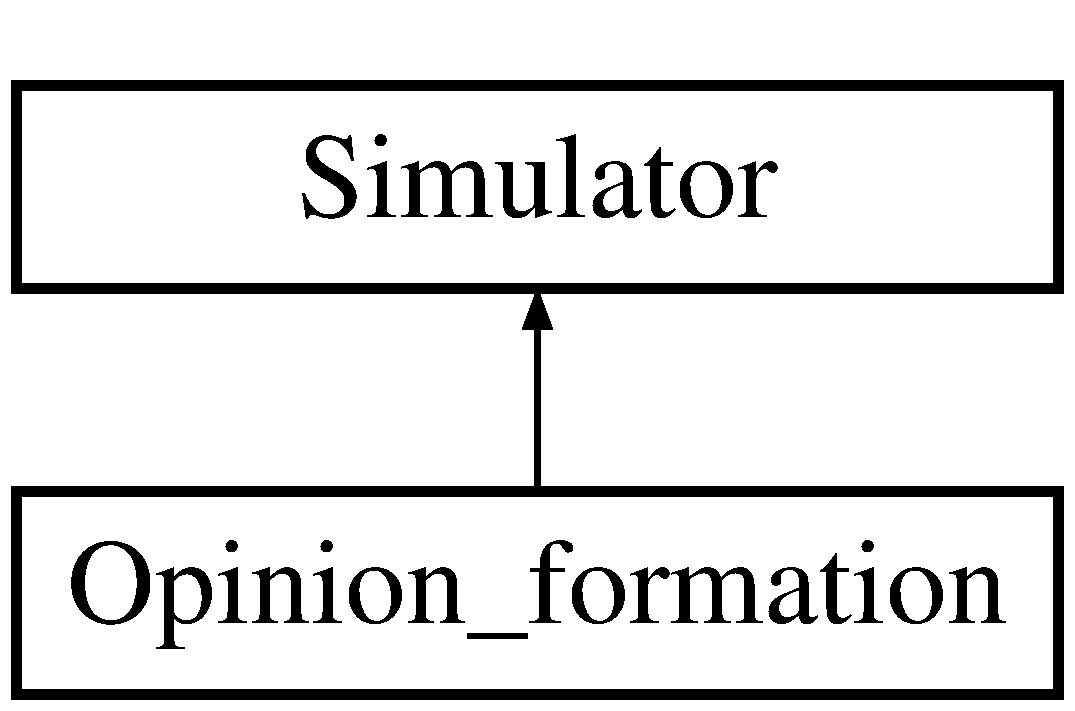
\includegraphics[height=2.000000cm]{classOpinion__formation}
\end{center}
\end{figure}
\subsection*{Public Member Functions}
\begin{DoxyCompactItemize}
\item 
\hypertarget{classOpinion__formation_a7509661b00bc038cf556ea8b4567f8dd}{}{\bfseries Opinion\+\_\+formation} (\hyperlink{classNetwork}{Network} $\ast$net, string \&filename)\label{classOpinion__formation_a7509661b00bc038cf556ea8b4567f8dd}

\item 
\hypertarget{classOpinion__formation_a0e3f268e479e5804935c19be5bf9adc8}{}{\bfseries Opinion\+\_\+formation} (vector$<$ \hyperlink{classNetwork}{Network} $\ast$ $>$ net\+\_\+list, string \&filename)\label{classOpinion__formation_a0e3f268e479e5804935c19be5bf9adc8}

\item 
\hypertarget{classOpinion__formation_ad3023ef5cec9c16c65d41a9570973ab8}{}void {\bfseries time\+\_\+step} ()\label{classOpinion__formation_ad3023ef5cec9c16c65d41a9570973ab8}

\item 
\hypertarget{classOpinion__formation_a17cd66c91458877408932302acdc5957}{}void {\bfseries run\+\_\+simulation} (int max\+\_\+time)\label{classOpinion__formation_a17cd66c91458877408932302acdc5957}

\item 
\hypertarget{classOpinion__formation_a85de0cfebe9e6d4b7e45daebdd79e7b4}{}void {\bfseries reset} ()\label{classOpinion__formation_a85de0cfebe9e6d4b7e45daebdd79e7b4}

\item 
\hypertarget{classOpinion__formation_a234809db4df362ca24c10dfa222aeb17}{}void {\bfseries summary} ()\label{classOpinion__formation_a234809db4df362ca24c10dfa222aeb17}

\end{DoxyCompactItemize}
\subsection*{Public Attributes}
\begin{DoxyCompactItemize}
\item 
\hypertarget{classOpinion__formation_a3050d046588c99ac730e4a00ffa4b631}{}ofstream {\bfseries outfile}\label{classOpinion__formation_a3050d046588c99ac730e4a00ffa4b631}

\end{DoxyCompactItemize}
\subsection*{Protected Attributes}
\begin{DoxyCompactItemize}
\item 
\hypertarget{classOpinion__formation_a4d8db8d1f1a9b635d88171788c9d1e38}{}double {\bfseries beta} =10\label{classOpinion__formation_a4d8db8d1f1a9b635d88171788c9d1e38}

\end{DoxyCompactItemize}


The documentation for this class was generated from the following file\+:\begin{DoxyCompactItemize}
\item 
Opinion\+\_\+formation.\+h\end{DoxyCompactItemize}

\hypertarget{classPercolation__Sim}{}\section{Percolation\+\_\+\+Sim Class Reference}
\label{classPercolation__Sim}\index{Percolation\+\_\+\+Sim@{Percolation\+\_\+\+Sim}}
Inheritance diagram for Percolation\+\_\+\+Sim\+:\begin{figure}[H]
\begin{center}
\leavevmode
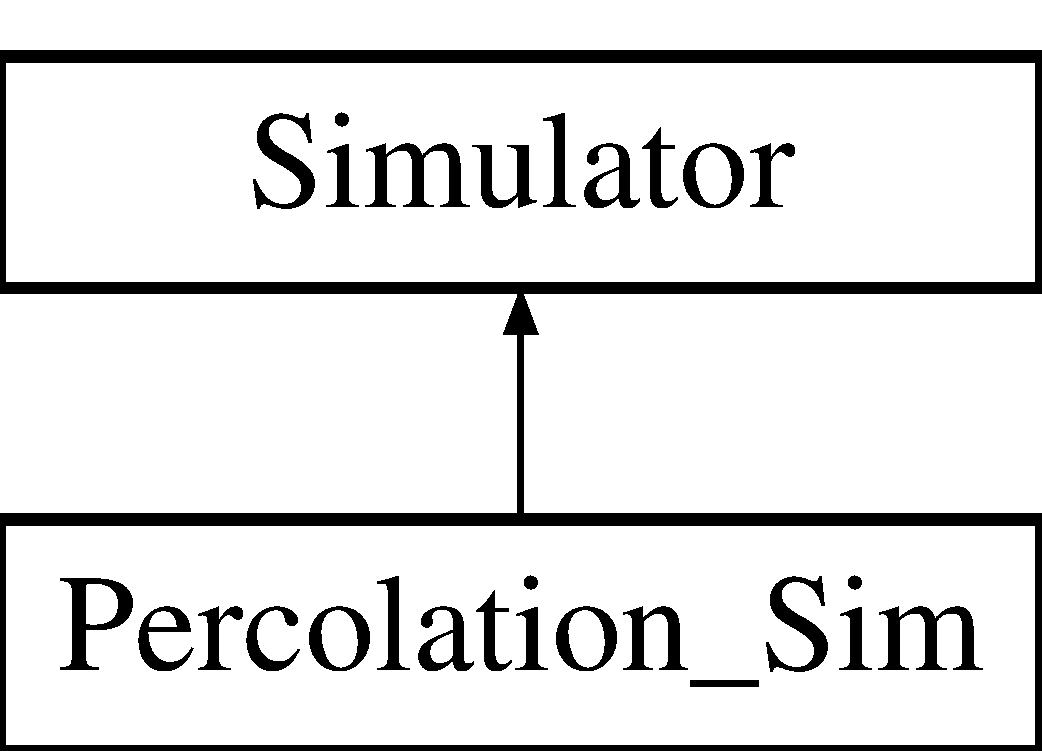
\includegraphics[height=2.000000cm]{classPercolation__Sim}
\end{center}
\end{figure}
\subsection*{Public Types}
\begin{DoxyCompactItemize}
\item 
\hypertarget{classPercolation__Sim_ae2805212eff0710bffa6cf55d0c31917}{}enum {\bfseries state\+Type} \{ {\bfseries S} =0, 
{\bfseries I} =1, 
{\bfseries R} =-\/1
 \}\label{classPercolation__Sim_ae2805212eff0710bffa6cf55d0c31917}

\end{DoxyCompactItemize}
\subsection*{Public Member Functions}
\begin{DoxyCompactItemize}
\item 
\hypertarget{classPercolation__Sim_a68dc8b2121f6f555fd99711867634618}{}{\bfseries Percolation\+\_\+\+Sim} (\hyperlink{classNetwork}{Network} $\ast$net)\label{classPercolation__Sim_a68dc8b2121f6f555fd99711867634618}

\item 
\hypertarget{classPercolation__Sim_a331fbf29f66960463f2c6f2caab3bdf3}{}void {\bfseries set\+\_\+transmissibility} (double t)\label{classPercolation__Sim_a331fbf29f66960463f2c6f2caab3bdf3}

\item 
\hypertarget{classPercolation__Sim_ab0334facd8aebdb7df20e778a9577d09}{}double {\bfseries expected\+\_\+\+R0} ()\label{classPercolation__Sim_ab0334facd8aebdb7df20e778a9577d09}

\item 
\hypertarget{classPercolation__Sim_a71a7cd862e374aa87e7ff11f872aab0b}{}vector$<$ \hyperlink{classNode}{Node} $\ast$ $>$ {\bfseries rand\+\_\+infect} (int n)\label{classPercolation__Sim_a71a7cd862e374aa87e7ff11f872aab0b}

\item 
\hypertarget{classPercolation__Sim_abab9361ad723b13011469509dbcdddf4}{}void {\bfseries step\+\_\+simulation} ()\label{classPercolation__Sim_abab9361ad723b13011469509dbcdddf4}

\item 
\hypertarget{classPercolation__Sim_ac4deb883b042d030130f2619c62a25e3}{}void {\bfseries run\+\_\+simulation} ()\label{classPercolation__Sim_ac4deb883b042d030130f2619c62a25e3}

\item 
\hypertarget{classPercolation__Sim_a0ee2603b7f5aca0a2f0af5a8650d1872}{}int {\bfseries count\+\_\+infected} ()\label{classPercolation__Sim_a0ee2603b7f5aca0a2f0af5a8650d1872}

\item 
\hypertarget{classPercolation__Sim_a925aba2a0dcdbf8406e76acc15b1fbf8}{}int {\bfseries epidemic\+\_\+size} ()\label{classPercolation__Sim_a925aba2a0dcdbf8406e76acc15b1fbf8}

\item 
\hypertarget{classPercolation__Sim_a966c4deb4da447e6ca946361a01b4f7b}{}void {\bfseries reset} ()\label{classPercolation__Sim_a966c4deb4da447e6ca946361a01b4f7b}

\item 
\hypertarget{classPercolation__Sim_aaad5cfb0f15994f76f68e050290680e1}{}void {\bfseries summary} ()\label{classPercolation__Sim_aaad5cfb0f15994f76f68e050290680e1}

\end{DoxyCompactItemize}
\subsection*{Public Attributes}
\begin{DoxyCompactItemize}
\item 
\hypertarget{classPercolation__Sim_a49395f0bb8d201ba759cc8283ca92595}{}float {\bfseries T}\label{classPercolation__Sim_a49395f0bb8d201ba759cc8283ca92595}

\end{DoxyCompactItemize}
\subsection*{Protected Attributes}
\begin{DoxyCompactItemize}
\item 
\hypertarget{classPercolation__Sim_a2d1e8339487c926fc6f1ae4ca6c70e81}{}vector$<$ \hyperlink{classNode}{Node} $\ast$ $>$ {\bfseries infected}\label{classPercolation__Sim_a2d1e8339487c926fc6f1ae4ca6c70e81}

\item 
\hypertarget{classPercolation__Sim_a493e6dfe3ee61cf8715724d2eb1d0437}{}vector$<$ \hyperlink{classNode}{Node} $\ast$ $>$ {\bfseries recovered}\label{classPercolation__Sim_a493e6dfe3ee61cf8715724d2eb1d0437}

\end{DoxyCompactItemize}


The documentation for this class was generated from the following file\+:\begin{DoxyCompactItemize}
\item 
Percolation\+\_\+\+Sim.\+h\end{DoxyCompactItemize}

\hypertarget{classRPlot}{}\section{R\+Plot Class Reference}
\label{classRPlot}\index{R\+Plot@{R\+Plot}}
\subsection*{Public Member Functions}
\begin{DoxyCompactItemize}
\item 
\hypertarget{classRPlot_a86981eba64a9b138a5856c76aa14059a}{}void {\bfseries define\+\_\+header} (string h)\label{classRPlot_a86981eba64a9b138a5856c76aa14059a}

\item 
\hypertarget{classRPlot_aa4e6d065ffc5cb6d234bb72a23563a38}{}void {\bfseries define\+\_\+footer} (string f)\label{classRPlot_aa4e6d065ffc5cb6d234bb72a23563a38}

\item 
\hypertarget{classRPlot_a0b0ce5474847d7b1947126c6975e07c4}{}void {\bfseries define} (string par, double val)\label{classRPlot_a0b0ce5474847d7b1947126c6975e07c4}

\item 
\hypertarget{classRPlot_a486fe81dc519208ef2243aa38346ac37}{}void {\bfseries define} (string par, string val)\label{classRPlot_a486fe81dc519208ef2243aa38346ac37}

\item 
\hypertarget{classRPlot_adc0785839f48e5b8cd8a15a26ed69aba}{}void {\bfseries set\+\_\+x} (vector$<$ double $>$ x)\label{classRPlot_adc0785839f48e5b8cd8a15a26ed69aba}

\item 
\hypertarget{classRPlot_aec0a33b9b55359e1245cadd26279544e}{}void {\bfseries set\+\_\+y} (vector$<$ double $>$ y, string color=\char`\"{}1\char`\"{}, string pch=\char`\"{}1\char`\"{}, string type=\char`\"{}p\char`\"{})\label{classRPlot_aec0a33b9b55359e1245cadd26279544e}

\item 
\hypertarget{classRPlot_ac2af6bb29d7a64f8b4a06f4529729350}{}void {\bfseries add\+\_\+y} (vector$<$ double $>$ y, string color=\char`\"{}1\char`\"{}, string pch=\char`\"{}1\char`\"{}, string type=\char`\"{}p\char`\"{})\label{classRPlot_ac2af6bb29d7a64f8b4a06f4529729350}

\item 
\hypertarget{classRPlot_ab83248b865eb569cc16023a0bbbf7353}{}int {\bfseries pdf} (string filename, double width=10, double height=7.\+5)\label{classRPlot_ab83248b865eb569cc16023a0bbbf7353}

\item 
\hypertarget{classRPlot_a68b6837eaf2fd5b0c507232cab2e8556}{}int {\bfseries png} (string filename, double width=1000, double height=750)\label{classRPlot_a68b6837eaf2fd5b0c507232cab2e8556}

\item 
\hypertarget{classRPlot_acb6587e142ae8f956b25df31df03ab68}{}int {\bfseries \+\_\+plotter} (string plot\+\_\+type, string filename, double width, double height)\label{classRPlot_acb6587e142ae8f956b25df31df03ab68}

\item 
\hypertarget{classRPlot_aad36764d50f156772b941724c2d5b3a4}{}void {\bfseries write\+\_\+datafile} (string filename)\label{classRPlot_aad36764d50f156772b941724c2d5b3a4}

\item 
\hypertarget{classRPlot_a825904f102a043e9c8324d4bee4e7fb8}{}string {\bfseries xlim} (vector$<$ double $>$ X, vector$<$ \hyperlink{classYseries}{Yseries} $\ast$ $>$ Y)\label{classRPlot_a825904f102a043e9c8324d4bee4e7fb8}

\item 
\hypertarget{classRPlot_a68d8faba8df754f11fd6d04d1f0cc61a}{}string {\bfseries ylim} (vector$<$ double $>$ X, vector$<$ \hyperlink{classYseries}{Yseries} $\ast$ $>$ Y)\label{classRPlot_a68d8faba8df754f11fd6d04d1f0cc61a}

\item 
\hypertarget{classRPlot_afab1cb327dcd2a9d575f800863ebece5}{}vector$<$ double $>$ {\bfseries determine\+\_\+limits} (vector$<$ \hyperlink{classYseries}{Yseries} $\ast$ $>$ Y)\label{classRPlot_afab1cb327dcd2a9d575f800863ebece5}

\end{DoxyCompactItemize}


The documentation for this class was generated from the following file\+:\begin{DoxyCompactItemize}
\item 
R\+Plot.\+h\end{DoxyCompactItemize}

\hypertarget{classSimulator}{}\section{Simulator Class Reference}
\label{classSimulator}\index{Simulator@{Simulator}}
Inheritance diagram for Simulator\+:\begin{figure}[H]
\begin{center}
\leavevmode
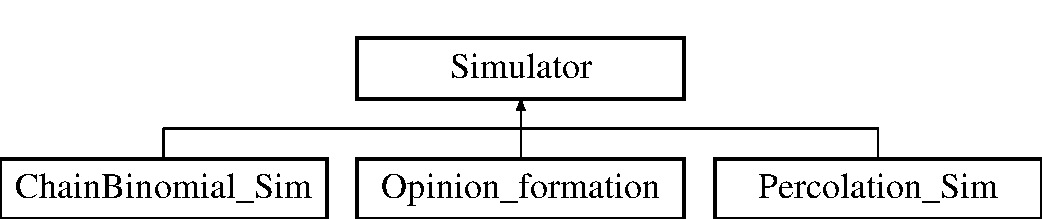
\includegraphics[height=2.000000cm]{classSimulator}
\end{center}
\end{figure}
\subsection*{Public Member Functions}
\begin{DoxyCompactItemize}
\item 
\hypertarget{classSimulator_afac88757024c1074b6b0c3c39c441010}{}{\bfseries Simulator} (\hyperlink{classNetwork}{Network} $\ast$net, string fname)\label{classSimulator_afac88757024c1074b6b0c3c39c441010}

\item 
\hypertarget{classSimulator_a476a63ef9b628c54d0129ffe270465ed}{}{\bfseries Simulator} (vector$<$ \hyperlink{classNetwork}{Network} $\ast$ $>$ net\+\_\+list, string fname)\label{classSimulator_a476a63ef9b628c54d0129ffe270465ed}

\item 
\hypertarget{classSimulator_a340d96c82d8ff7786949a620dee2ee53}{}void {\bfseries set\+\_\+network} (\hyperlink{classNetwork}{Network} $\ast$net)\label{classSimulator_a340d96c82d8ff7786949a620dee2ee53}

\item 
\hypertarget{classSimulator_a0255e53faefcf2acd6b594551f7e3a92}{}\hyperlink{classNetwork}{Network} $\ast$ {\bfseries network} ()\label{classSimulator_a0255e53faefcf2acd6b594551f7e3a92}

\item 
\hypertarget{classSimulator_a775d86392b65bf43adadba7a8c6286fd}{}int {\bfseries get\+\_\+time} ()\label{classSimulator_a775d86392b65bf43adadba7a8c6286fd}

\item 
\hypertarget{classSimulator_a97fa0d0068e759f345ff06cc5436fc3a}{}void {\bfseries reset\+\_\+time} ()\label{classSimulator_a97fa0d0068e759f345ff06cc5436fc3a}

\item 
\hypertarget{classSimulator_a20c0e44c291569c4ea17cc93f7b069bf}{}void {\bfseries set\+\_\+all\+\_\+nodes\+\_\+to\+\_\+state} (state\+Type s)\label{classSimulator_a20c0e44c291569c4ea17cc93f7b069bf}

\item 
\hypertarget{classSimulator_a9b6c9f8c97a6142c39b95bb3d77cf18c}{}void {\bfseries set\+\_\+these\+\_\+nodes\+\_\+to\+\_\+state} (vector$<$ \hyperlink{classNode}{Node} $\ast$ $>$ nodes, state\+Type s)\label{classSimulator_a9b6c9f8c97a6142c39b95bb3d77cf18c}

\item 
\hypertarget{classSimulator_a61a761f7efaf7b63b7a8dff3ae50f00f}{}vector$<$ \hyperlink{classNode}{Node} $\ast$ $>$ {\bfseries rand\+\_\+choose\+\_\+nodes} (int n)\label{classSimulator_a61a761f7efaf7b63b7a8dff3ae50f00f}

\item 
\hypertarget{classSimulator_a1b4bad3cfa952e283ac1576c2b9357a8}{}vector$<$ \hyperlink{classNode}{Node} $\ast$ $>$ {\bfseries rand\+\_\+set\+\_\+nodes\+\_\+to\+\_\+state} (int n, state\+Type state)\label{classSimulator_a1b4bad3cfa952e283ac1576c2b9357a8}

\item 
\hypertarget{classSimulator_a3bee1aeade42b904c9a561e0e4c84460}{}virtual void {\bfseries time\+\_\+step} ()\label{classSimulator_a3bee1aeade42b904c9a561e0e4c84460}

\item 
\hypertarget{classSimulator_accb74d40c16c3a6a7f658e5d272bdf0c}{}virtual void {\bfseries run\+\_\+simulation} ()\label{classSimulator_accb74d40c16c3a6a7f658e5d272bdf0c}

\item 
\hypertarget{classSimulator_a51fba2398daa6f380fa4034856735491}{}virtual int {\bfseries count\+\_\+infected} ()\label{classSimulator_a51fba2398daa6f380fa4034856735491}

\item 
\hypertarget{classSimulator_a23ddae46561995fccb3d5a769efa1294}{}virtual void {\bfseries reset} ()\label{classSimulator_a23ddae46561995fccb3d5a769efa1294}

\end{DoxyCompactItemize}
\subsection*{Public Attributes}
\begin{DoxyCompactItemize}
\item 
\hypertarget{classSimulator_aa81e60ca4246da452d64dddb70beb33f}{}int {\bfseries time}\label{classSimulator_aa81e60ca4246da452d64dddb70beb33f}

\item 
\hypertarget{classSimulator_a1570947a7c2c40c45f24a0d599463328}{}\hyperlink{classNetwork}{Network} $\ast$ {\bfseries net}\label{classSimulator_a1570947a7c2c40c45f24a0d599463328}

\item 
\hypertarget{classSimulator_a0f168636a3de4d3336a23606f3111173}{}\hyperlink{classMTRand}{M\+T\+Rand} $\ast$ {\bfseries mtrand}\label{classSimulator_a0f168636a3de4d3336a23606f3111173}

\item 
\hypertarget{classSimulator_a7fd4ec3cb930229a61fc31f9ba4a4ab2}{}vector$<$ \hyperlink{classNetwork}{Network} $\ast$ $>$ {\bfseries net\+\_\+list}\label{classSimulator_a7fd4ec3cb930229a61fc31f9ba4a4ab2}

\item 
\hypertarget{classSimulator_a413c5a4e5af6ada7fe66b7689678f087}{}string {\bfseries fname}\label{classSimulator_a413c5a4e5af6ada7fe66b7689678f087}

\end{DoxyCompactItemize}
\subsection*{Protected Attributes}
\begin{DoxyCompactItemize}
\item 
\hypertarget{classSimulator_a1a287cb00e5388a7866b5e4f5a35a137}{}time\+\_\+t {\bfseries starttime}\label{classSimulator_a1a287cb00e5388a7866b5e4f5a35a137}

\end{DoxyCompactItemize}


The documentation for this class was generated from the following file\+:\begin{DoxyCompactItemize}
\item 
Simulator.\+h\end{DoxyCompactItemize}

\hypertarget{classSIR}{}\section{S\+I\+R Class Reference}
\label{classSIR}\index{S\+I\+R@{S\+I\+R}}
Inheritance diagram for S\+I\+R\+:\begin{figure}[H]
\begin{center}
\leavevmode
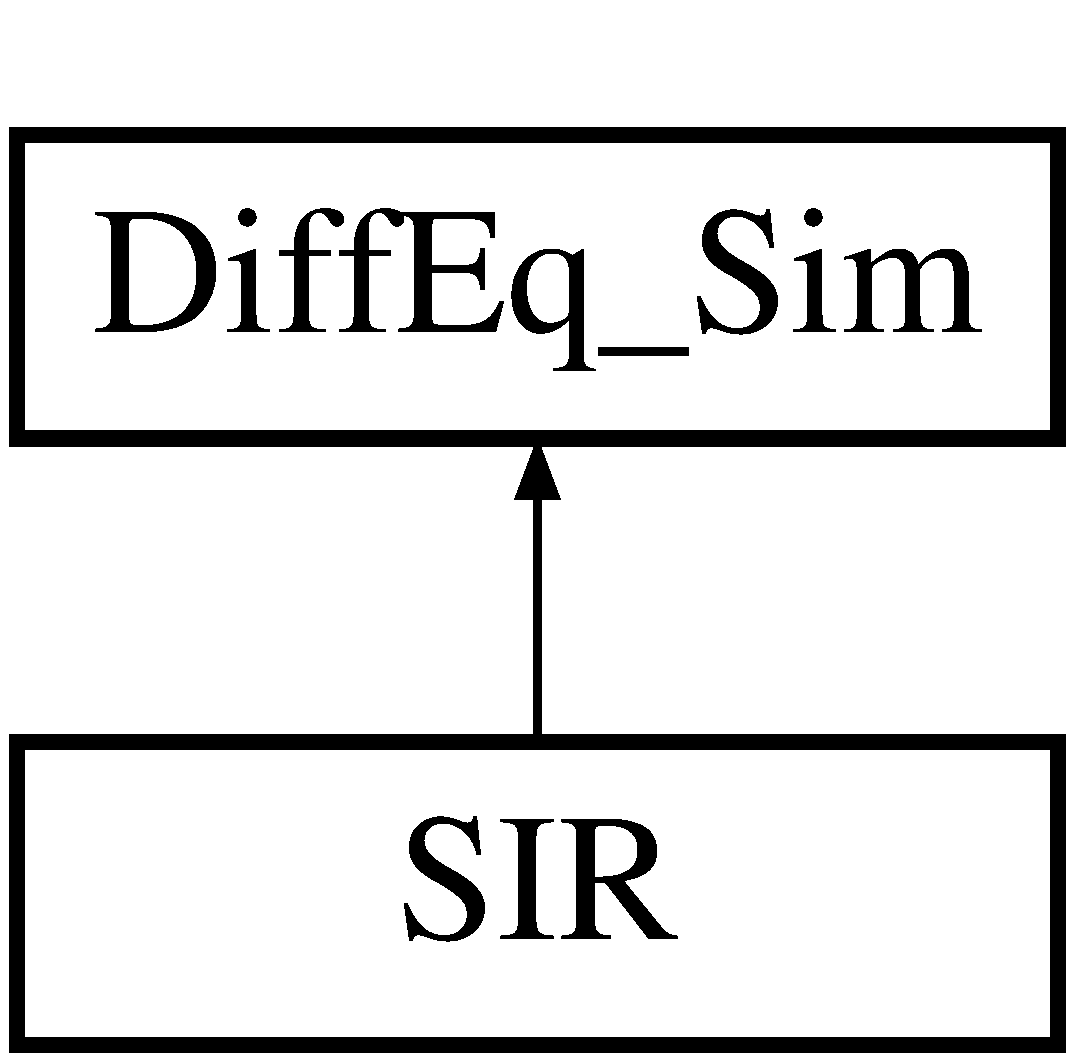
\includegraphics[height=2.000000cm]{classSIR}
\end{center}
\end{figure}
\subsection*{Public Member Functions}
\begin{DoxyCompactItemize}
\item 
\hypertarget{classSIR_a398344819c9e0e32947922efb4c0433d}{}{\bfseries S\+I\+R} (double b, double g)\label{classSIR_a398344819c9e0e32947922efb4c0433d}

\item 
\hypertarget{classSIR_af7839bbe96120c50f2ce5bc6a4ea5fd9}{}void {\bfseries initialize} (double S, double I, double R)\label{classSIR_af7839bbe96120c50f2ce5bc6a4ea5fd9}

\item 
\hypertarget{classSIR_aee7ad4c67c83fcdb7848fa184199466c}{}void {\bfseries derivative} (double const y\mbox{[}$\,$\mbox{]}, double dydt\mbox{[}$\,$\mbox{]})\label{classSIR_aee7ad4c67c83fcdb7848fa184199466c}

\end{DoxyCompactItemize}
\subsection*{Additional Inherited Members}


The documentation for this class was generated from the following file\+:\begin{DoxyCompactItemize}
\item 
S\+I\+R\+\_\+\+Sim.\+h\end{DoxyCompactItemize}

\hypertarget{classTrigger}{}\section{Trigger Class Reference}
\label{classTrigger}\index{Trigger@{Trigger}}


The documentation for this class was generated from the following file\+:\begin{DoxyCompactItemize}
\item 
Intervention.\+h\end{DoxyCompactItemize}

\hypertarget{classYseries}{}\section{Yseries Class Reference}
\label{classYseries}\index{Yseries@{Yseries}}
\subsection*{Public Member Functions}
\begin{DoxyCompactItemize}
\item 
\hypertarget{classYseries_a9be497f36c55fce41a55da4e01aa9572}{}{\bfseries Yseries} (vector$<$ double $>$ d, string c, string p, string t)\label{classYseries_a9be497f36c55fce41a55da4e01aa9572}

\item 
\hypertarget{classYseries_a5bc0a282eb4db0040de12409703fe586}{}int {\bfseries size} ()\label{classYseries_a5bc0a282eb4db0040de12409703fe586}

\item 
\hypertarget{classYseries_a2868b1ad13eb474d4a02dd949d1eb203}{}vector$<$ double $>$ {\bfseries data} ()\label{classYseries_a2868b1ad13eb474d4a02dd949d1eb203}

\item 
\hypertarget{classYseries_a34767aa102b85ed47738ce525e7963b2}{}double {\bfseries data} (int i)\label{classYseries_a34767aa102b85ed47738ce525e7963b2}

\item 
\hypertarget{classYseries_a7cc70f3ff8ba1bd3e78bae175099ab05}{}string {\bfseries col} ()\label{classYseries_a7cc70f3ff8ba1bd3e78bae175099ab05}

\item 
\hypertarget{classYseries_abf97d4c566049b0cd5d8a9c6fd7a04df}{}string {\bfseries pch} ()\label{classYseries_abf97d4c566049b0cd5d8a9c6fd7a04df}

\item 
\hypertarget{classYseries_a25b60b539632f2b2f88d6f7759b8e946}{}string {\bfseries type} ()\label{classYseries_a25b60b539632f2b2f88d6f7759b8e946}

\end{DoxyCompactItemize}
\subsection*{Public Attributes}
\begin{DoxyCompactItemize}
\item 
\hypertarget{classYseries_aeb321ec45633adf99bb54b70ff77ffef}{}vector$<$ double $>$ {\bfseries D}\label{classYseries_aeb321ec45633adf99bb54b70ff77ffef}

\item 
\hypertarget{classYseries_a4b1beb6b072129a31a13cd59cd1d8359}{}string {\bfseries C}\label{classYseries_a4b1beb6b072129a31a13cd59cd1d8359}

\item 
\hypertarget{classYseries_a9a6fb62d1d73bbaf9f5bc5e0797389f9}{}string {\bfseries P}\label{classYseries_a9a6fb62d1d73bbaf9f5bc5e0797389f9}

\item 
\hypertarget{classYseries_acfa4f5a5f1259fb07c0265e8983df5bd}{}string {\bfseries T}\label{classYseries_acfa4f5a5f1259fb07c0265e8983df5bd}

\end{DoxyCompactItemize}


The documentation for this class was generated from the following file\+:\begin{DoxyCompactItemize}
\item 
R\+Plot.\+h\end{DoxyCompactItemize}

%--- End generated contents ---

% Index
\backmatter
\newpage
\phantomsection
\clearemptydoublepage
\addcontentsline{toc}{chapter}{Index}
\printindex

\end{document}
